\documentclass[11pt,a4paper]{article}

% Manuscript of the systematic review with meta-analysis, FDI vs FCM.
% RULE: no number is typed by hand. Every number comes from \val{key}, defined
% in generati/numeri.tex, which scripts/manoscritto_meta.py generates from
% state.sqlite, 30-Dati/ and 50-Metanalisi/. Tables in generati/ are generated too.

\usepackage[utf8]{inputenc}
\usepackage[T1]{fontenc}
\usepackage{lmodern}
\usepackage[english]{babel}
\usepackage[margin=2.2cm]{geometry}
\usepackage{setspace}
\usepackage{microtype}
\usepackage{amsmath,amssymb}
\usepackage{booktabs,tabularx,array,longtable}
\usepackage{pdflscape}
\usepackage[table]{xcolor}
\usepackage{graphicx}
\usepackage{tikz}
\usetikzlibrary{positioning,arrows.meta,calc}
\usepackage{caption}
\captionsetup{font=small,labelfont=bf}
\usepackage{enumitem}
\setlist{nosep,leftmargin=*}
\usepackage[numbers,sort&compress]{natbib}
\usepackage{lineno}
\usepackage[hidelinks]{hyperref}
\usepackage{doi}

\graphicspath{{../../50-Metanalisi/output/forest/}}
% generato da scripts/manoscritto_meta.py — non modificare a mano
\makeatletter
\@namedef{val@P1.estesa.RD.diff_1000}{$-$369}
\@namedef{val@P1.estesa.RD.diff_1000_inf}{$-$510}
\@namedef{val@P1.estesa.RD.diff_1000_sup}{$-$227}
\@namedef{val@P1.estesa.RD.eventi_fcm}{29/61}
\@namedef{val@P1.estesa.RD.eventi_fdi}{6/62}
\@namedef{val@P1.estesa.RD.i2}{0}
\@namedef{val@P1.estesa.RD.ic_inf}{$-$0.51}
\@namedef{val@P1.estesa.RD.ic_sup}{$-$0.23}
\@namedef{val@P1.estesa.RD.k}{2}
\@namedef{val@P1.estesa.RD.p}{$<$0.001}
\@namedef{val@P1.estesa.RD.partecipanti}{123}
\@namedef{val@P1.estesa.RD.q}{0.00}
\@namedef{val@P1.estesa.RD.q_p}{1.00}
\@namedef{val@P1.estesa.RD.rischio_fcm_1000}{475}
\@namedef{val@P1.estesa.RD.stima}{$-$0.37}
\@namedef{val@P1.estesa.RD.tau2}{0.000}
\@namedef{val@P1.estesa.affiancato-k-5.mh-effetti-fissi-senza-correzione.RR.eventi_fcm}{29/61}
\@namedef{val@P1.estesa.affiancato-k-5.mh-effetti-fissi-senza-correzione.RR.eventi_fdi}{6/62}
\@namedef{val@P1.estesa.affiancato-k-5.mh-effetti-fissi-senza-correzione.RR.k}{2}
\@namedef{val@P1.estesa.affiancato-k-5.reml-hksj-senza-correzione.RR.eventi_fcm}{29/61}
\@namedef{val@P1.estesa.affiancato-k-5.reml-hksj-senza-correzione.RR.eventi_fdi}{6/62}
\@namedef{val@P1.estesa.affiancato-k-5.reml-hksj-senza-correzione.RR.k}{2}
\@namedef{val@P1.estesa.sensibilit-1-solo-rob-basso.mh-effetti-fissi-doppi-zeri-inclusi.RD.k}{0}
\@namedef{val@P1.estesa.sensibilit-3-soglia-esatta.mh-effetti-fissi-doppi-zeri-inclusi.RD.eventi_fcm}{29/61}
\@namedef{val@P1.estesa.sensibilit-3-soglia-esatta.mh-effetti-fissi-doppi-zeri-inclusi.RD.eventi_fdi}{6/62}
\@namedef{val@P1.estesa.sensibilit-3-soglia-esatta.mh-effetti-fissi-doppi-zeri-inclusi.RD.k}{2}
\@namedef{val@P1.estesa.sensibilit-4-senza-produttore.mh-effetti-fissi-doppi-zeri-inclusi.RD.k}{0}
\@namedef{val@P1.estesa.sensibilit-5-senza-dati-solo-da-registro-abstract.mh-effetti-fissi-doppi-zeri-inclusi.RD.eventi_fcm}{29/61}
\@namedef{val@P1.estesa.sensibilit-5-senza-dati-solo-da-registro-abstract.mh-effetti-fissi-doppi-zeri-inclusi.RD.eventi_fdi}{6/62}
\@namedef{val@P1.estesa.sensibilit-5-senza-dati-solo-da-registro-abstract.mh-effetti-fissi-doppi-zeri-inclusi.RD.k}{2}
\@namedef{val@P1.estesa.sensibilit-correzione-0-5.reml-hksj-0-5-solo-ai-trial-con-zeri.RR.eventi_fcm}{29/61}
\@namedef{val@P1.estesa.sensibilit-correzione-0-5.reml-hksj-0-5-solo-ai-trial-con-zeri.RR.eventi_fdi}{6/62}
\@namedef{val@P1.estesa.sensibilit-correzione-0-5.reml-hksj-0-5-solo-ai-trial-con-zeri.RR.i2}{0}
\@namedef{val@P1.estesa.sensibilit-correzione-0-5.reml-hksj-0-5-solo-ai-trial-con-zeri.RR.ic_inf}{0.096}
\@namedef{val@P1.estesa.sensibilit-correzione-0-5.reml-hksj-0-5-solo-ai-trial-con-zeri.RR.ic_sup}{0.46}
\@namedef{val@P1.estesa.sensibilit-correzione-0-5.reml-hksj-0-5-solo-ai-trial-con-zeri.RR.k}{1}
\@namedef{val@P1.estesa.sensibilit-correzione-0-5.reml-hksj-0-5-solo-ai-trial-con-zeri.RR.p}{$<$0.001}
\@namedef{val@P1.estesa.sensibilit-correzione-0-5.reml-hksj-0-5-solo-ai-trial-con-zeri.RR.q}{0.00}
\@namedef{val@P1.estesa.sensibilit-correzione-0-5.reml-hksj-0-5-solo-ai-trial-con-zeri.RR.q_p}{1.00}
\@namedef{val@P1.estesa.sensibilit-correzione-0-5.reml-hksj-0-5-solo-ai-trial-con-zeri.RR.stima}{0.21}
\@namedef{val@P1.estesa.sensibilit-correzione-0-5.reml-hksj-0-5-solo-ai-trial-con-zeri.RR.tau2}{0.000}
\@namedef{val@P1.primaria.RR.diff_1000}{$-$599}
\@namedef{val@P1.primaria.RR.diff_1000_inf}{$-$622}
\@namedef{val@P1.primaria.RR.diff_1000_sup}{$-$566}
\@namedef{val@P1.primaria.RR.eventi_fcm}{121/190}
\@namedef{val@P1.primaria.RR.eventi_fdi}{15/200}
\@namedef{val@P1.primaria.RR.i2}{0}
\@namedef{val@P1.primaria.RR.ic_inf}{0.085}
\@namedef{val@P1.primaria.RR.ic_sup}{0.17}
\@namedef{val@P1.primaria.RR.k}{4}
\@namedef{val@P1.primaria.RR.p}{$<$0.001}
\@namedef{val@P1.primaria.RR.partecipanti}{364}
\@namedef{val@P1.primaria.RR.pi_inf}{0.085}
\@namedef{val@P1.primaria.RR.pi_sup}{0.17}
\@namedef{val@P1.primaria.RR.q}{0.54}
\@namedef{val@P1.primaria.RR.q_p}{0.91}
\@namedef{val@P1.primaria.RR.rischio_fcm_1000}{680}
\@namedef{val@P1.primaria.RR.rischio_fdi_1000}{81}
\@namedef{val@P1.primaria.RR.stima}{0.12}
\@namedef{val@P1.primaria.RR.tau2}{0.000}
\@namedef{val@P1.primaria.affiancato-k-5.mh-effetti-fissi-senza-correzione.RR.eventi_fcm}{121/190}
\@namedef{val@P1.primaria.affiancato-k-5.mh-effetti-fissi-senza-correzione.RR.eventi_fdi}{15/200}
\@namedef{val@P1.primaria.affiancato-k-5.mh-effetti-fissi-senza-correzione.RR.i2}{0}
\@namedef{val@P1.primaria.affiancato-k-5.mh-effetti-fissi-senza-correzione.RR.ic_inf}{0.072}
\@namedef{val@P1.primaria.affiancato-k-5.mh-effetti-fissi-senza-correzione.RR.ic_sup}{0.19}
\@namedef{val@P1.primaria.affiancato-k-5.mh-effetti-fissi-senza-correzione.RR.k}{4}
\@namedef{val@P1.primaria.affiancato-k-5.mh-effetti-fissi-senza-correzione.RR.p}{$<$0.001}
\@namedef{val@P1.primaria.affiancato-k-5.mh-effetti-fissi-senza-correzione.RR.q}{0.54}
\@namedef{val@P1.primaria.affiancato-k-5.mh-effetti-fissi-senza-correzione.RR.q_p}{0.91}
\@namedef{val@P1.primaria.affiancato-k-5.mh-effetti-fissi-senza-correzione.RR.stima}{0.12}
\@namedef{val@P1.primaria.affiancato-k-5.mh-effetti-fissi-senza-correzione.RR.tau2}{0.000}
\@namedef{val@P1.primaria.sensibilit-1-solo-rob-basso.reml-hksj-senza-correzione.RR.k}{0}
\@namedef{val@P1.primaria.sensibilit-2-effetti-fissi-iv.inverso-della-varianza-effetti-fissi.RR.eventi_fcm}{121/190}
\@namedef{val@P1.primaria.sensibilit-2-effetti-fissi-iv.inverso-della-varianza-effetti-fissi.RR.eventi_fdi}{15/200}
\@namedef{val@P1.primaria.sensibilit-2-effetti-fissi-iv.inverso-della-varianza-effetti-fissi.RR.i2}{0}
\@namedef{val@P1.primaria.sensibilit-2-effetti-fissi-iv.inverso-della-varianza-effetti-fissi.RR.ic_inf}{0.073}
\@namedef{val@P1.primaria.sensibilit-2-effetti-fissi-iv.inverso-della-varianza-effetti-fissi.RR.ic_sup}{0.20}
\@namedef{val@P1.primaria.sensibilit-2-effetti-fissi-iv.inverso-della-varianza-effetti-fissi.RR.k}{4}
\@namedef{val@P1.primaria.sensibilit-2-effetti-fissi-iv.inverso-della-varianza-effetti-fissi.RR.p}{$<$0.001}
\@namedef{val@P1.primaria.sensibilit-2-effetti-fissi-iv.inverso-della-varianza-effetti-fissi.RR.q}{0.54}
\@namedef{val@P1.primaria.sensibilit-2-effetti-fissi-iv.inverso-della-varianza-effetti-fissi.RR.q_p}{0.91}
\@namedef{val@P1.primaria.sensibilit-2-effetti-fissi-iv.inverso-della-varianza-effetti-fissi.RR.stima}{0.12}
\@namedef{val@P1.primaria.sensibilit-2-effetti-fissi-iv.inverso-della-varianza-effetti-fissi.RR.tau2}{0.000}
\@namedef{val@P1.primaria.sensibilit-3-soglia-esatta.reml-hksj-senza-correzione.RR.eventi_fcm}{121/190}
\@namedef{val@P1.primaria.sensibilit-3-soglia-esatta.reml-hksj-senza-correzione.RR.eventi_fdi}{15/200}
\@namedef{val@P1.primaria.sensibilit-3-soglia-esatta.reml-hksj-senza-correzione.RR.k}{5}
\@namedef{val@P1.primaria.sensibilit-4-senza-produttore.reml-hksj-senza-correzione.RR.k}{0}
\@namedef{val@P1.primaria.sensibilit-5-senza-dati-solo-da-registro-abstract.reml-hksj-senza-correzione.RR.eventi_fcm}{121/190}
\@namedef{val@P1.primaria.sensibilit-5-senza-dati-solo-da-registro-abstract.reml-hksj-senza-correzione.RR.eventi_fdi}{15/200}
\@namedef{val@P1.primaria.sensibilit-5-senza-dati-solo-da-registro-abstract.reml-hksj-senza-correzione.RR.k}{5}
\@namedef{val@P1.primaria.sensibilit-correzione-0-5.reml-hksj-0-5-solo-ai-trial-con-zeri.RR.eventi_fcm}{121/190}
\@namedef{val@P1.primaria.sensibilit-correzione-0-5.reml-hksj-0-5-solo-ai-trial-con-zeri.RR.eventi_fdi}{15/200}
\@namedef{val@P1.primaria.sensibilit-correzione-0-5.reml-hksj-0-5-solo-ai-trial-con-zeri.RR.i2}{0}
\@namedef{val@P1.primaria.sensibilit-correzione-0-5.reml-hksj-0-5-solo-ai-trial-con-zeri.RR.ic_inf}{0.085}
\@namedef{val@P1.primaria.sensibilit-correzione-0-5.reml-hksj-0-5-solo-ai-trial-con-zeri.RR.ic_sup}{0.17}
\@namedef{val@P1.primaria.sensibilit-correzione-0-5.reml-hksj-0-5-solo-ai-trial-con-zeri.RR.k}{4}
\@namedef{val@P1.primaria.sensibilit-correzione-0-5.reml-hksj-0-5-solo-ai-trial-con-zeri.RR.p}{$<$0.001}
\@namedef{val@P1.primaria.sensibilit-correzione-0-5.reml-hksj-0-5-solo-ai-trial-con-zeri.RR.pi_inf}{0.085}
\@namedef{val@P1.primaria.sensibilit-correzione-0-5.reml-hksj-0-5-solo-ai-trial-con-zeri.RR.pi_sup}{0.17}
\@namedef{val@P1.primaria.sensibilit-correzione-0-5.reml-hksj-0-5-solo-ai-trial-con-zeri.RR.q}{0.54}
\@namedef{val@P1.primaria.sensibilit-correzione-0-5.reml-hksj-0-5-solo-ai-trial-con-zeri.RR.q_p}{0.91}
\@namedef{val@P1.primaria.sensibilit-correzione-0-5.reml-hksj-0-5-solo-ai-trial-con-zeri.RR.stima}{0.12}
\@namedef{val@P1.primaria.sensibilit-correzione-0-5.reml-hksj-0-5-solo-ai-trial-con-zeri.RR.tau2}{0.000}
\@namedef{val@P1.primaria.sottogruppi-popolazione.reml-hksj-senza-correzione.RR.eventi_fcm}{121/190}
\@namedef{val@P1.primaria.sottogruppi-popolazione.reml-hksj-senza-correzione.RR.eventi_fdi}{15/200}
\@namedef{val@P1.primaria.sottogruppi-popolazione.reml-hksj-senza-correzione.RR.k}{5}
\@namedef{val@P1.primaria.sottogruppi-test-schema-dose.reml-hksj-senza-correzione.RR.eventi_fcm}{121/178}
\@namedef{val@P1.primaria.sottogruppi-test-schema-dose.reml-hksj-senza-correzione.RR.eventi_fdi}{15/186}
\@namedef{val@P1.primaria.sottogruppi-test-schema-dose.reml-hksj-senza-correzione.RR.k}{4}
\@namedef{val@P1.primaria.sottogruppi-test-schema-dose.reml-hksj-senza-correzione.RR.q}{2.87}
\@namedef{val@P1.primaria.sottogruppi-test-schema-dose.reml-hksj-senza-correzione.RR.q_p}{0.09}
\@namedef{val@P1.primaria.sottogruppo-schema-dose-fdi-singola-fcm-frazionata.reml-hksj-senza-correzione.RR.eventi_fcm}{87/117}
\@namedef{val@P1.primaria.sottogruppo-schema-dose-fdi-singola-fcm-frazionata.reml-hksj-senza-correzione.RR.eventi_fdi}{10/125}
\@namedef{val@P1.primaria.sottogruppo-schema-dose-fdi-singola-fcm-frazionata.reml-hksj-senza-correzione.RR.i2}{0}
\@namedef{val@P1.primaria.sottogruppo-schema-dose-fdi-singola-fcm-frazionata.reml-hksj-senza-correzione.RR.ic_inf}{0.087}
\@namedef{val@P1.primaria.sottogruppo-schema-dose-fdi-singola-fcm-frazionata.reml-hksj-senza-correzione.RR.ic_sup}{0.13}
\@namedef{val@P1.primaria.sottogruppo-schema-dose-fdi-singola-fcm-frazionata.reml-hksj-senza-correzione.RR.k}{2}
\@namedef{val@P1.primaria.sottogruppo-schema-dose-fdi-singola-fcm-frazionata.reml-hksj-senza-correzione.RR.p}{0.0048}
\@namedef{val@P1.primaria.sottogruppo-schema-dose-fdi-singola-fcm-frazionata.reml-hksj-senza-correzione.RR.q}{0.00}
\@namedef{val@P1.primaria.sottogruppo-schema-dose-fdi-singola-fcm-frazionata.reml-hksj-senza-correzione.RR.q_p}{0.96}
\@namedef{val@P1.primaria.sottogruppo-schema-dose-fdi-singola-fcm-frazionata.reml-hksj-senza-correzione.RR.stima}{0.11}
\@namedef{val@P1.primaria.sottogruppo-schema-dose-fdi-singola-fcm-frazionata.reml-hksj-senza-correzione.RR.tau2}{0.000}
\@namedef{val@P1.primaria.sottogruppo-schema-dose-stesso-schema.reml-hksj-senza-correzione.RR.eventi_fcm}{34/61}
\@namedef{val@P1.primaria.sottogruppo-schema-dose-stesso-schema.reml-hksj-senza-correzione.RR.eventi_fdi}{5/61}
\@namedef{val@P1.primaria.sottogruppo-schema-dose-stesso-schema.reml-hksj-senza-correzione.RR.i2}{0}
\@namedef{val@P1.primaria.sottogruppo-schema-dose-stesso-schema.reml-hksj-senza-correzione.RR.ic_inf}{0.013}
\@namedef{val@P1.primaria.sottogruppo-schema-dose-stesso-schema.reml-hksj-senza-correzione.RR.ic_sup}{1.63}
\@namedef{val@P1.primaria.sottogruppo-schema-dose-stesso-schema.reml-hksj-senza-correzione.RR.k}{2}
\@namedef{val@P1.primaria.sottogruppo-schema-dose-stesso-schema.reml-hksj-senza-correzione.RR.p}{0.06}
\@namedef{val@P1.primaria.sottogruppo-schema-dose-stesso-schema.reml-hksj-senza-correzione.RR.q}{0.18}
\@namedef{val@P1.primaria.sottogruppo-schema-dose-stesso-schema.reml-hksj-senza-correzione.RR.q_p}{0.67}
\@namedef{val@P1.primaria.sottogruppo-schema-dose-stesso-schema.reml-hksj-senza-correzione.RR.stima}{0.15}
\@namedef{val@P1.primaria.sottogruppo-schema-dose-stesso-schema.reml-hksj-senza-correzione.RR.tau2}{0.000}
\@namedef{val@S1.primaria.OR.diff_1000}{$-$99}
\@namedef{val@S1.primaria.OR.diff_1000_inf}{$-$108}
\@namedef{val@S1.primaria.OR.diff_1000_sup}{$-$71}
\@namedef{val@S1.primaria.OR.eventi_fcm}{13/210}
\@namedef{val@S1.primaria.OR.eventi_fdi}{0/217}
\@namedef{val@S1.primaria.OR.i2}{0}
\@namedef{val@S1.primaria.OR.ic_inf}{0.037}
\@namedef{val@S1.primaria.OR.ic_sup}{0.34}
\@namedef{val@S1.primaria.OR.k}{2}
\@namedef{val@S1.primaria.OR.p}{$<$0.001}
\@namedef{val@S1.primaria.OR.partecipanti}{239}
\@namedef{val@S1.primaria.OR.q}{0.00}
\@namedef{val@S1.primaria.OR.q_p}{0.99}
\@namedef{val@S1.primaria.OR.rischio_fcm_1000}{113}
\@namedef{val@S1.primaria.OR.rischio_fdi_1000}{14}
\@namedef{val@S1.primaria.OR.stima}{0.11}
\@namedef{val@S1.primaria.OR.tau2}{0.000}
\@namedef{val@S1.primaria.RD.diff_1000}{$-$63}
\@namedef{val@S1.primaria.RD.diff_1000_inf}{$-$96}
\@namedef{val@S1.primaria.RD.diff_1000_sup}{$-$30}
\@namedef{val@S1.primaria.RD.eventi_fcm}{13/210}
\@namedef{val@S1.primaria.RD.eventi_fdi}{0/217}
\@namedef{val@S1.primaria.RD.i2}{59}
\@namedef{val@S1.primaria.RD.ic_inf}{$-$0.096}
\@namedef{val@S1.primaria.RD.ic_sup}{$-$0.03}
\@namedef{val@S1.primaria.RD.k}{3}
\@namedef{val@S1.primaria.RD.p}{$<$0.001}
\@namedef{val@S1.primaria.RD.partecipanti}{427}
\@namedef{val@S1.primaria.RD.q}{2.46}
\@namedef{val@S1.primaria.RD.q_p}{0.12}
\@namedef{val@S1.primaria.RD.rischio_fcm_1000}{62}
\@namedef{val@S1.primaria.RD.stima}{$-$0.063}
\@namedef{val@S1.primaria.RD.tau2}{0.000}
\@namedef{val@S1.primaria.affiancato-k-5.mh-effetti-fissi-senza-correzione.RR.eventi_fcm}{13/210}
\@namedef{val@S1.primaria.affiancato-k-5.mh-effetti-fissi-senza-correzione.RR.eventi_fdi}{0/217}
\@namedef{val@S1.primaria.affiancato-k-5.mh-effetti-fissi-senza-correzione.RR.k}{2}
\@namedef{val@S1.primaria.affiancato-k-5.mh-effetti-fissi-senza-correzione.RR.tau2}{0.000}
\@namedef{val@S1.primaria.affiancato-k-5.reml-hksj-senza-correzione.RR.eventi_fcm}{13/210}
\@namedef{val@S1.primaria.affiancato-k-5.reml-hksj-senza-correzione.RR.eventi_fdi}{0/217}
\@namedef{val@S1.primaria.affiancato-k-5.reml-hksj-senza-correzione.RR.k}{3}
\@namedef{val@S1.primaria.sensibilit-1-solo-rob-basso.mh-effetti-fissi-doppi-zeri-inclusi.RD.k}{0}
\@namedef{val@S1.primaria.sensibilit-1-solo-rob-basso.peto.OR.k}{0}
\@namedef{val@S1.primaria.sensibilit-3-soglia-esatta.mh-effetti-fissi-doppi-zeri-inclusi.RD.eventi_fcm}{13/115}
\@namedef{val@S1.primaria.sensibilit-3-soglia-esatta.mh-effetti-fissi-doppi-zeri-inclusi.RD.eventi_fdi}{0/124}
\@namedef{val@S1.primaria.sensibilit-3-soglia-esatta.mh-effetti-fissi-doppi-zeri-inclusi.RD.i2}{0}
\@namedef{val@S1.primaria.sensibilit-3-soglia-esatta.mh-effetti-fissi-doppi-zeri-inclusi.RD.ic_inf}{$-$0.17}
\@namedef{val@S1.primaria.sensibilit-3-soglia-esatta.mh-effetti-fissi-doppi-zeri-inclusi.RD.ic_sup}{$-$0.055}
\@namedef{val@S1.primaria.sensibilit-3-soglia-esatta.mh-effetti-fissi-doppi-zeri-inclusi.RD.k}{2}
\@namedef{val@S1.primaria.sensibilit-3-soglia-esatta.mh-effetti-fissi-doppi-zeri-inclusi.RD.p}{$<$0.001}
\@namedef{val@S1.primaria.sensibilit-3-soglia-esatta.mh-effetti-fissi-doppi-zeri-inclusi.RD.q}{0.04}
\@namedef{val@S1.primaria.sensibilit-3-soglia-esatta.mh-effetti-fissi-doppi-zeri-inclusi.RD.q_p}{0.85}
\@namedef{val@S1.primaria.sensibilit-3-soglia-esatta.mh-effetti-fissi-doppi-zeri-inclusi.RD.stima}{$-$0.11}
\@namedef{val@S1.primaria.sensibilit-3-soglia-esatta.mh-effetti-fissi-doppi-zeri-inclusi.RD.tau2}{0.000}
\@namedef{val@S1.primaria.sensibilit-3-soglia-esatta.peto.OR.eventi_fcm}{13/115}
\@namedef{val@S1.primaria.sensibilit-3-soglia-esatta.peto.OR.eventi_fdi}{0/124}
\@namedef{val@S1.primaria.sensibilit-3-soglia-esatta.peto.OR.i2}{0}
\@namedef{val@S1.primaria.sensibilit-3-soglia-esatta.peto.OR.ic_inf}{0.037}
\@namedef{val@S1.primaria.sensibilit-3-soglia-esatta.peto.OR.ic_sup}{0.34}
\@namedef{val@S1.primaria.sensibilit-3-soglia-esatta.peto.OR.k}{2}
\@namedef{val@S1.primaria.sensibilit-3-soglia-esatta.peto.OR.p}{$<$0.001}
\@namedef{val@S1.primaria.sensibilit-3-soglia-esatta.peto.OR.q}{0.00}
\@namedef{val@S1.primaria.sensibilit-3-soglia-esatta.peto.OR.q_p}{0.99}
\@namedef{val@S1.primaria.sensibilit-3-soglia-esatta.peto.OR.stima}{0.11}
\@namedef{val@S1.primaria.sensibilit-3-soglia-esatta.peto.OR.tau2}{0.000}
\@namedef{val@S1.primaria.sensibilit-4-senza-produttore.mh-effetti-fissi-doppi-zeri-inclusi.RD.eventi_fcm}{0/95}
\@namedef{val@S1.primaria.sensibilit-4-senza-produttore.mh-effetti-fissi-doppi-zeri-inclusi.RD.eventi_fdi}{0/93}
\@namedef{val@S1.primaria.sensibilit-4-senza-produttore.mh-effetti-fissi-doppi-zeri-inclusi.RD.k}{1}
\@namedef{val@S1.primaria.sensibilit-4-senza-produttore.peto.OR.eventi_fcm}{0/95}
\@namedef{val@S1.primaria.sensibilit-4-senza-produttore.peto.OR.eventi_fdi}{0/93}
\@namedef{val@S1.primaria.sensibilit-4-senza-produttore.peto.OR.k}{1}
\@namedef{val@S1.primaria.sensibilit-5-senza-dati-solo-da-registro-abstract.mh-effetti-fissi-doppi-zeri-inclusi.RD.eventi_fcm}{0/95}
\@namedef{val@S1.primaria.sensibilit-5-senza-dati-solo-da-registro-abstract.mh-effetti-fissi-doppi-zeri-inclusi.RD.eventi_fdi}{0/93}
\@namedef{val@S1.primaria.sensibilit-5-senza-dati-solo-da-registro-abstract.mh-effetti-fissi-doppi-zeri-inclusi.RD.k}{1}
\@namedef{val@S1.primaria.sensibilit-5-senza-dati-solo-da-registro-abstract.peto.OR.eventi_fcm}{0/95}
\@namedef{val@S1.primaria.sensibilit-5-senza-dati-solo-da-registro-abstract.peto.OR.eventi_fdi}{0/93}
\@namedef{val@S1.primaria.sensibilit-5-senza-dati-solo-da-registro-abstract.peto.OR.k}{1}
\@namedef{val@S1.primaria.sensibilit-correzione-0-5.reml-hksj-0-5-solo-ai-trial-con-zeri.RR.eventi_fcm}{13/210}
\@namedef{val@S1.primaria.sensibilit-correzione-0-5.reml-hksj-0-5-solo-ai-trial-con-zeri.RR.eventi_fdi}{0/217}
\@namedef{val@S1.primaria.sensibilit-correzione-0-5.reml-hksj-0-5-solo-ai-trial-con-zeri.RR.i2}{0}
\@namedef{val@S1.primaria.sensibilit-correzione-0-5.reml-hksj-0-5-solo-ai-trial-con-zeri.RR.ic_inf}{0.03}
\@namedef{val@S1.primaria.sensibilit-correzione-0-5.reml-hksj-0-5-solo-ai-trial-con-zeri.RR.ic_sup}{0.15}
\@namedef{val@S1.primaria.sensibilit-correzione-0-5.reml-hksj-0-5-solo-ai-trial-con-zeri.RR.k}{2}
\@namedef{val@S1.primaria.sensibilit-correzione-0-5.reml-hksj-0-5-solo-ai-trial-con-zeri.RR.p}{0.01}
\@namedef{val@S1.primaria.sensibilit-correzione-0-5.reml-hksj-0-5-solo-ai-trial-con-zeri.RR.q}{0.00}
\@namedef{val@S1.primaria.sensibilit-correzione-0-5.reml-hksj-0-5-solo-ai-trial-con-zeri.RR.q_p}{0.95}
\@namedef{val@S1.primaria.sensibilit-correzione-0-5.reml-hksj-0-5-solo-ai-trial-con-zeri.RR.stima}{0.066}
\@namedef{val@S1.primaria.sensibilit-correzione-0-5.reml-hksj-0-5-solo-ai-trial-con-zeri.RR.tau2}{0.000}
\@namedef{val@S2.estesa.RR.eventi_fcm}{1/12}
\@namedef{val@S2.estesa.RR.eventi_fdi}{1/14}
\@namedef{val@S2.estesa.RR.k}{1}
\@namedef{val@S2.estesa.RR.partecipanti}{26}
\@namedef{val@S2.primaria.RR.eventi_fcm}{3/95}
\@namedef{val@S2.primaria.RR.eventi_fdi}{2/93}
\@namedef{val@S2.primaria.RR.k}{1}
\@namedef{val@S2.primaria.RR.partecipanti}{188}
\@namedef{val@S3.primaria.RR.diff_1000}{$-$298}
\@namedef{val@S3.primaria.RR.diff_1000_inf}{$-$310}
\@namedef{val@S3.primaria.RR.diff_1000_sup}{$-$262}
\@namedef{val@S3.primaria.RR.eventi_fcm}{54/171}
\@namedef{val@S3.primaria.RR.eventi_fdi}{3/171}
\@namedef{val@S3.primaria.RR.i2}{56}
\@namedef{val@S3.primaria.RR.ic_inf}{0.018}
\@namedef{val@S3.primaria.RR.ic_sup}{0.17}
\@namedef{val@S3.primaria.RR.k}{4}
\@namedef{val@S3.primaria.RR.p}{$<$0.001}
\@namedef{val@S3.primaria.RR.partecipanti}{342}
\@namedef{val@S3.primaria.RR.q}{6.83}
\@namedef{val@S3.primaria.RR.q_p}{0.077}
\@namedef{val@S3.primaria.RR.rischio_fcm_1000}{316}
\@namedef{val@S3.primaria.RR.rischio_fdi_1000}{17}
\@namedef{val@S3.primaria.RR.stima}{0.055}
\@namedef{val@S3.primaria.RR.tau2}{0.000}
\@namedef{val@S3.primaria.affiancato-k-5.reml-hksj-senza-correzione.RR.eventi_fcm}{54/171}
\@namedef{val@S3.primaria.affiancato-k-5.reml-hksj-senza-correzione.RR.eventi_fdi}{3/171}
\@namedef{val@S3.primaria.affiancato-k-5.reml-hksj-senza-correzione.RR.i2}{39}
\@namedef{val@S3.primaria.affiancato-k-5.reml-hksj-senza-correzione.RR.ic_inf}{0.0056}
\@namedef{val@S3.primaria.affiancato-k-5.reml-hksj-senza-correzione.RR.ic_sup}{5.34}
\@namedef{val@S3.primaria.affiancato-k-5.reml-hksj-senza-correzione.RR.k}{3}
\@namedef{val@S3.primaria.affiancato-k-5.reml-hksj-senza-correzione.RR.p}{0.16}
\@namedef{val@S3.primaria.affiancato-k-5.reml-hksj-senza-correzione.RR.pi_inf}{0.0011}
\@namedef{val@S3.primaria.affiancato-k-5.reml-hksj-senza-correzione.RR.pi_sup}{28.54}
\@namedef{val@S3.primaria.affiancato-k-5.reml-hksj-senza-correzione.RR.q}{3.25}
\@namedef{val@S3.primaria.affiancato-k-5.reml-hksj-senza-correzione.RR.q_p}{0.20}
\@namedef{val@S3.primaria.affiancato-k-5.reml-hksj-senza-correzione.RR.stima}{0.17}
\@namedef{val@S3.primaria.affiancato-k-5.reml-hksj-senza-correzione.RR.tau2}{0.772}
\@namedef{val@S3.primaria.sensibilit-1-solo-rob-basso.mh-effetti-fissi-senza-correzione.RR.k}{0}
\@namedef{val@S3.primaria.sensibilit-2-effetti-fissi-iv.inverso-della-varianza-effetti-fissi.RR.eventi_fcm}{54/171}
\@namedef{val@S3.primaria.sensibilit-2-effetti-fissi-iv.inverso-della-varianza-effetti-fissi.RR.eventi_fdi}{3/171}
\@namedef{val@S3.primaria.sensibilit-2-effetti-fissi-iv.inverso-della-varianza-effetti-fissi.RR.i2}{38}
\@namedef{val@S3.primaria.sensibilit-2-effetti-fissi-iv.inverso-della-varianza-effetti-fissi.RR.ic_inf}{0.048}
\@namedef{val@S3.primaria.sensibilit-2-effetti-fissi-iv.inverso-della-varianza-effetti-fissi.RR.ic_sup}{0.56}
\@namedef{val@S3.primaria.sensibilit-2-effetti-fissi-iv.inverso-della-varianza-effetti-fissi.RR.k}{3}
\@namedef{val@S3.primaria.sensibilit-2-effetti-fissi-iv.inverso-della-varianza-effetti-fissi.RR.p}{0.0039}
\@namedef{val@S3.primaria.sensibilit-2-effetti-fissi-iv.inverso-della-varianza-effetti-fissi.RR.q}{3.25}
\@namedef{val@S3.primaria.sensibilit-2-effetti-fissi-iv.inverso-della-varianza-effetti-fissi.RR.q_p}{0.20}
\@namedef{val@S3.primaria.sensibilit-2-effetti-fissi-iv.inverso-della-varianza-effetti-fissi.RR.stima}{0.16}
\@namedef{val@S3.primaria.sensibilit-2-effetti-fissi-iv.inverso-della-varianza-effetti-fissi.RR.tau2}{0.000}
\@namedef{val@S3.primaria.sensibilit-3-soglia-esatta.mh-effetti-fissi-senza-correzione.RR.eventi_fcm}{54/171}
\@namedef{val@S3.primaria.sensibilit-3-soglia-esatta.mh-effetti-fissi-senza-correzione.RR.eventi_fdi}{3/171}
\@namedef{val@S3.primaria.sensibilit-3-soglia-esatta.mh-effetti-fissi-senza-correzione.RR.k}{4}
\@namedef{val@S3.primaria.sensibilit-4-senza-produttore.mh-effetti-fissi-senza-correzione.RR.k}{0}
\@namedef{val@S3.primaria.sensibilit-5-senza-dati-solo-da-registro-abstract.mh-effetti-fissi-senza-correzione.RR.eventi_fcm}{54/171}
\@namedef{val@S3.primaria.sensibilit-5-senza-dati-solo-da-registro-abstract.mh-effetti-fissi-senza-correzione.RR.eventi_fdi}{3/171}
\@namedef{val@S3.primaria.sensibilit-5-senza-dati-solo-da-registro-abstract.mh-effetti-fissi-senza-correzione.RR.k}{4}
\@namedef{val@S3.primaria.sensibilit-correzione-0-5.reml-hksj-0-5-solo-ai-trial-con-zeri.RR.eventi_fcm}{54/171}
\@namedef{val@S3.primaria.sensibilit-correzione-0-5.reml-hksj-0-5-solo-ai-trial-con-zeri.RR.eventi_fdi}{3/171}
\@namedef{val@S3.primaria.sensibilit-correzione-0-5.reml-hksj-0-5-solo-ai-trial-con-zeri.RR.i2}{41}
\@namedef{val@S3.primaria.sensibilit-correzione-0-5.reml-hksj-0-5-solo-ai-trial-con-zeri.RR.ic_inf}{0.0097}
\@namedef{val@S3.primaria.sensibilit-correzione-0-5.reml-hksj-0-5-solo-ai-trial-con-zeri.RR.ic_sup}{1.33}
\@namedef{val@S3.primaria.sensibilit-correzione-0-5.reml-hksj-0-5-solo-ai-trial-con-zeri.RR.k}{4}
\@namedef{val@S3.primaria.sensibilit-correzione-0-5.reml-hksj-0-5-solo-ai-trial-con-zeri.RR.p}{0.07}
\@namedef{val@S3.primaria.sensibilit-correzione-0-5.reml-hksj-0-5-solo-ai-trial-con-zeri.RR.pi_inf}{0.0022}
\@namedef{val@S3.primaria.sensibilit-correzione-0-5.reml-hksj-0-5-solo-ai-trial-con-zeri.RR.pi_sup}{5.90}
\@namedef{val@S3.primaria.sensibilit-correzione-0-5.reml-hksj-0-5-solo-ai-trial-con-zeri.RR.q}{5.19}
\@namedef{val@S3.primaria.sensibilit-correzione-0-5.reml-hksj-0-5-solo-ai-trial-con-zeri.RR.q_p}{0.16}
\@namedef{val@S3.primaria.sensibilit-correzione-0-5.reml-hksj-0-5-solo-ai-trial-con-zeri.RR.stima}{0.11}
\@namedef{val@S3.primaria.sensibilit-correzione-0-5.reml-hksj-0-5-solo-ai-trial-con-zeri.RR.tau2}{0.943}
\@namedef{val@S3.primaria.sottogruppi-popolazione.mh-effetti-fissi-senza-correzione.RR.eventi_fcm}{54/171}
\@namedef{val@S3.primaria.sottogruppi-popolazione.mh-effetti-fissi-senza-correzione.RR.eventi_fdi}{3/171}
\@namedef{val@S3.primaria.sottogruppi-popolazione.mh-effetti-fissi-senza-correzione.RR.k}{4}
\@namedef{val@S3.primaria.sottogruppi-test-schema-dose.mh-effetti-fissi-senza-correzione.RR.eventi_fcm}{54/171}
\@namedef{val@S3.primaria.sottogruppi-test-schema-dose.mh-effetti-fissi-senza-correzione.RR.eventi_fdi}{3/171}
\@namedef{val@S3.primaria.sottogruppi-test-schema-dose.mh-effetti-fissi-senza-correzione.RR.k}{4}
\@namedef{val@S3.primaria.sottogruppi-test-schema-dose.mh-effetti-fissi-senza-correzione.RR.q}{5.49}
\@namedef{val@S3.primaria.sottogruppi-test-schema-dose.mh-effetti-fissi-senza-correzione.RR.q_p}{0.019}
\@namedef{val@S3.primaria.sottogruppo-schema-dose-fdi-singola-fcm-frazionata.mh-effetti-fissi-senza-correzione.RR.eventi_fcm}{49/114}
\@namedef{val@S3.primaria.sottogruppo-schema-dose-fdi-singola-fcm-frazionata.mh-effetti-fissi-senza-correzione.RR.eventi_fdi}{1/117}
\@namedef{val@S3.primaria.sottogruppo-schema-dose-fdi-singola-fcm-frazionata.mh-effetti-fissi-senza-correzione.RR.i2}{0}
\@namedef{val@S3.primaria.sottogruppo-schema-dose-fdi-singola-fcm-frazionata.mh-effetti-fissi-senza-correzione.RR.ic_inf}{0.0028}
\@namedef{val@S3.primaria.sottogruppo-schema-dose-fdi-singola-fcm-frazionata.mh-effetti-fissi-senza-correzione.RR.ic_sup}{0.14}
\@namedef{val@S3.primaria.sottogruppo-schema-dose-fdi-singola-fcm-frazionata.mh-effetti-fissi-senza-correzione.RR.k}{2}
\@namedef{val@S3.primaria.sottogruppo-schema-dose-fdi-singola-fcm-frazionata.mh-effetti-fissi-senza-correzione.RR.p}{$<$0.001}
\@namedef{val@S3.primaria.sottogruppo-schema-dose-fdi-singola-fcm-frazionata.mh-effetti-fissi-senza-correzione.RR.q}{0.51}
\@namedef{val@S3.primaria.sottogruppo-schema-dose-fdi-singola-fcm-frazionata.mh-effetti-fissi-senza-correzione.RR.q_p}{0.47}
\@namedef{val@S3.primaria.sottogruppo-schema-dose-fdi-singola-fcm-frazionata.mh-effetti-fissi-senza-correzione.RR.stima}{0.02}
\@namedef{val@S3.primaria.sottogruppo-schema-dose-fdi-singola-fcm-frazionata.mh-effetti-fissi-senza-correzione.RR.tau2}{0.000}
\@namedef{val@S3.primaria.sottogruppo-schema-dose-stesso-schema.mh-effetti-fissi-senza-correzione.RR.eventi_fcm}{5/57}
\@namedef{val@S3.primaria.sottogruppo-schema-dose-stesso-schema.mh-effetti-fissi-senza-correzione.RR.eventi_fdi}{2/54}
\@namedef{val@S3.primaria.sottogruppo-schema-dose-stesso-schema.mh-effetti-fissi-senza-correzione.RR.i2}{0}
\@namedef{val@S3.primaria.sottogruppo-schema-dose-stesso-schema.mh-effetti-fissi-senza-correzione.RR.ic_inf}{0.084}
\@namedef{val@S3.primaria.sottogruppo-schema-dose-stesso-schema.mh-effetti-fissi-senza-correzione.RR.ic_sup}{1.91}
\@namedef{val@S3.primaria.sottogruppo-schema-dose-stesso-schema.mh-effetti-fissi-senza-correzione.RR.k}{2}
\@namedef{val@S3.primaria.sottogruppo-schema-dose-stesso-schema.mh-effetti-fissi-senza-correzione.RR.p}{0.25}
\@namedef{val@S3.primaria.sottogruppo-schema-dose-stesso-schema.mh-effetti-fissi-senza-correzione.RR.q}{0.13}
\@namedef{val@S3.primaria.sottogruppo-schema-dose-stesso-schema.mh-effetti-fissi-senza-correzione.RR.q_p}{0.72}
\@namedef{val@S3.primaria.sottogruppo-schema-dose-stesso-schema.mh-effetti-fissi-senza-correzione.RR.stima}{0.40}
\@namedef{val@S3.primaria.sottogruppo-schema-dose-stesso-schema.mh-effetti-fissi-senza-correzione.RR.tau2}{0.000}
\@namedef{val@S4.primaria.MD.i2}{0}
\@namedef{val@S4.primaria.MD.ic_inf}{0.24}
\@namedef{val@S4.primaria.MD.ic_sup}{0.49}
\@namedef{val@S4.primaria.MD.k}{2}
\@namedef{val@S4.primaria.MD.p}{0.02}
\@namedef{val@S4.primaria.MD.partecipanti}{231}
\@namedef{val@S4.primaria.MD.q}{0.08}
\@namedef{val@S4.primaria.MD.q_p}{0.77}
\@namedef{val@S4.primaria.MD.stima}{0.36}
\@namedef{val@S4.primaria.MD.tau2}{0.000}
\@namedef{val@S4.primaria.affiancato-k-5-sens-2.inverso-della-varianza-effetti-fissi.MD.i2}{0}
\@namedef{val@S4.primaria.affiancato-k-5-sens-2.inverso-della-varianza-effetti-fissi.MD.ic_inf}{0.30}
\@namedef{val@S4.primaria.affiancato-k-5-sens-2.inverso-della-varianza-effetti-fissi.MD.ic_sup}{0.43}
\@namedef{val@S4.primaria.affiancato-k-5-sens-2.inverso-della-varianza-effetti-fissi.MD.k}{2}
\@namedef{val@S4.primaria.affiancato-k-5-sens-2.inverso-della-varianza-effetti-fissi.MD.p}{$<$0.001}
\@namedef{val@S4.primaria.affiancato-k-5-sens-2.inverso-della-varianza-effetti-fissi.MD.q}{0.08}
\@namedef{val@S4.primaria.affiancato-k-5-sens-2.inverso-della-varianza-effetti-fissi.MD.q_p}{0.77}
\@namedef{val@S4.primaria.affiancato-k-5-sens-2.inverso-della-varianza-effetti-fissi.MD.stima}{0.36}
\@namedef{val@S4.primaria.affiancato-k-5-sens-2.inverso-della-varianza-effetti-fissi.MD.tau2}{0.000}
\@namedef{val@S6.estesa.RR.eventi_fcm}{1/189}
\@namedef{val@S6.estesa.RR.eventi_fdi}{0/188}
\@namedef{val@S6.estesa.RR.k}{2}
\@namedef{val@S6.estesa.RR.partecipanti}{377}
\@namedef{val@S6.primaria.RR.diff_1000}{$-$1}
\@namedef{val@S6.primaria.RR.diff_1000_inf}{$-$2}
\@namedef{val@S6.primaria.RR.diff_1000_sup}{4}
\@namedef{val@S6.primaria.RR.eventi_fcm}{3/1697}
\@namedef{val@S6.primaria.RR.eventi_fdi}{1/1708}
\@namedef{val@S6.primaria.RR.i2}{0}
\@namedef{val@S6.primaria.RR.ic_inf}{0.033}
\@namedef{val@S6.primaria.RR.ic_sup}{3.02}
\@namedef{val@S6.primaria.RR.k}{3}
\@namedef{val@S6.primaria.RR.p}{0.32}
\@namedef{val@S6.primaria.RR.partecipanti}{3147}
\@namedef{val@S6.primaria.RR.q}{1.97}
\@namedef{val@S6.primaria.RR.q_p}{0.37}
\@namedef{val@S6.primaria.RR.rischio_fcm_1000}{2}
\@namedef{val@S6.primaria.RR.rischio_fdi_1000}{1}
\@namedef{val@S6.primaria.RR.stima}{0.32}
\@namedef{val@S6.primaria.RR.tau2}{0.000}
\@namedef{val@S6.primaria.affiancato-k-5.reml-hksj-senza-correzione.RR.eventi_fcm}{3/1697}
\@namedef{val@S6.primaria.affiancato-k-5.reml-hksj-senza-correzione.RR.eventi_fdi}{1/1708}
\@namedef{val@S6.primaria.affiancato-k-5.reml-hksj-senza-correzione.RR.k}{5}
\@namedef{val@S6.primaria.sensibilit-1-solo-rob-basso.mh-effetti-fissi-senza-correzione.RR.k}{0}
\@namedef{val@S6.primaria.sensibilit-4-senza-produttore.mh-effetti-fissi-senza-correzione.RR.eventi_fcm}{1/1580}
\@namedef{val@S6.primaria.sensibilit-4-senza-produttore.mh-effetti-fissi-senza-correzione.RR.eventi_fdi}{0/1583}
\@namedef{val@S6.primaria.sensibilit-4-senza-produttore.mh-effetti-fissi-senza-correzione.RR.k}{3}
\@namedef{val@S6.primaria.sensibilit-5-senza-dati-solo-da-registro-abstract.mh-effetti-fissi-senza-correzione.RR.eventi_fcm}{1/1580}
\@namedef{val@S6.primaria.sensibilit-5-senza-dati-solo-da-registro-abstract.mh-effetti-fissi-senza-correzione.RR.eventi_fdi}{0/1583}
\@namedef{val@S6.primaria.sensibilit-5-senza-dati-solo-da-registro-abstract.mh-effetti-fissi-senza-correzione.RR.k}{3}
\@namedef{val@S6.primaria.sensibilit-correzione-0-5.reml-hksj-0-5-solo-ai-trial-con-zeri.RR.eventi_fcm}{3/1697}
\@namedef{val@S6.primaria.sensibilit-correzione-0-5.reml-hksj-0-5-solo-ai-trial-con-zeri.RR.eventi_fdi}{1/1708}
\@namedef{val@S6.primaria.sensibilit-correzione-0-5.reml-hksj-0-5-solo-ai-trial-con-zeri.RR.i2}{0}
\@namedef{val@S6.primaria.sensibilit-correzione-0-5.reml-hksj-0-5-solo-ai-trial-con-zeri.RR.ic_inf}{0.015}
\@namedef{val@S6.primaria.sensibilit-correzione-0-5.reml-hksj-0-5-solo-ai-trial-con-zeri.RR.ic_sup}{19.35}
\@namedef{val@S6.primaria.sensibilit-correzione-0-5.reml-hksj-0-5-solo-ai-trial-con-zeri.RR.k}{3}
\@namedef{val@S6.primaria.sensibilit-correzione-0-5.reml-hksj-0-5-solo-ai-trial-con-zeri.RR.p}{0.53}
\@namedef{val@S6.primaria.sensibilit-correzione-0-5.reml-hksj-0-5-solo-ai-trial-con-zeri.RR.pi_inf}{0.015}
\@namedef{val@S6.primaria.sensibilit-correzione-0-5.reml-hksj-0-5-solo-ai-trial-con-zeri.RR.pi_sup}{19.35}
\@namedef{val@S6.primaria.sensibilit-correzione-0-5.reml-hksj-0-5-solo-ai-trial-con-zeri.RR.q}{1.63}
\@namedef{val@S6.primaria.sensibilit-correzione-0-5.reml-hksj-0-5-solo-ai-trial-con-zeri.RR.q_p}{0.44}
\@namedef{val@S6.primaria.sensibilit-correzione-0-5.reml-hksj-0-5-solo-ai-trial-con-zeri.RR.stima}{0.54}
\@namedef{val@S6.primaria.sensibilit-correzione-0-5.reml-hksj-0-5-solo-ai-trial-con-zeri.RR.tau2}{0.000}
\@namedef{val@S6.primaria.sensibilit-glmm.glmm-um-fs.OR.eventi_fcm}{3/1568}
\@namedef{val@S6.primaria.sensibilit-glmm.glmm-um-fs.OR.eventi_fdi}{1/1579}
\@namedef{val@S6.primaria.sensibilit-glmm.glmm-um-fs.OR.i2}{0}
\@namedef{val@S6.primaria.sensibilit-glmm.glmm-um-fs.OR.ic_inf}{0.032}
\@namedef{val@S6.primaria.sensibilit-glmm.glmm-um-fs.OR.ic_sup}{3.03}
\@namedef{val@S6.primaria.sensibilit-glmm.glmm-um-fs.OR.k}{3}
\@namedef{val@S6.primaria.sensibilit-glmm.glmm-um-fs.OR.p}{0.32}
\@namedef{val@S6.primaria.sensibilit-glmm.glmm-um-fs.OR.stima}{0.31}
\@namedef{val@S6.primaria.sensibilit-glmm.glmm-um-fs.OR.tau2}{0.000}
\@namedef{val@S6.primaria.sensibilit-mh-effetti-fissi-doppi-zeri-inclusi.mh-effetti-fissi-doppi-zeri-inclusi.RD.eventi_fcm}{3/1697}
\@namedef{val@S6.primaria.sensibilit-mh-effetti-fissi-doppi-zeri-inclusi.mh-effetti-fissi-doppi-zeri-inclusi.RD.eventi_fdi}{1/1708}
\@namedef{val@S6.primaria.sensibilit-mh-effetti-fissi-doppi-zeri-inclusi.mh-effetti-fissi-doppi-zeri-inclusi.RD.i2}{11}
\@namedef{val@S6.primaria.sensibilit-mh-effetti-fissi-doppi-zeri-inclusi.mh-effetti-fissi-doppi-zeri-inclusi.RD.ic_inf}{$-$0.0036}
\@namedef{val@S6.primaria.sensibilit-mh-effetti-fissi-doppi-zeri-inclusi.mh-effetti-fissi-doppi-zeri-inclusi.RD.ic_sup}{0.0011}
\@namedef{val@S6.primaria.sensibilit-mh-effetti-fissi-doppi-zeri-inclusi.mh-effetti-fissi-doppi-zeri-inclusi.RD.k}{5}
\@namedef{val@S6.primaria.sensibilit-mh-effetti-fissi-doppi-zeri-inclusi.mh-effetti-fissi-doppi-zeri-inclusi.RD.p}{0.29}
\@namedef{val@S6.primaria.sensibilit-mh-effetti-fissi-doppi-zeri-inclusi.mh-effetti-fissi-doppi-zeri-inclusi.RD.q}{2.25}
\@namedef{val@S6.primaria.sensibilit-mh-effetti-fissi-doppi-zeri-inclusi.mh-effetti-fissi-doppi-zeri-inclusi.RD.q_p}{0.33}
\@namedef{val@S6.primaria.sensibilit-mh-effetti-fissi-doppi-zeri-inclusi.mh-effetti-fissi-doppi-zeri-inclusi.RD.stima}{$-$0.0012}
\@namedef{val@S6.primaria.sensibilit-mh-effetti-fissi-doppi-zeri-inclusi.mh-effetti-fissi-doppi-zeri-inclusi.RD.tau2}{0.000}
\@namedef{val@S6.primaria.sensibilit-peto.peto.OR.eventi_fcm}{3/1697}
\@namedef{val@S6.primaria.sensibilit-peto.peto.OR.eventi_fdi}{1/1708}
\@namedef{val@S6.primaria.sensibilit-peto.peto.OR.i2}{34}
\@namedef{val@S6.primaria.sensibilit-peto.peto.OR.ic_inf}{0.049}
\@namedef{val@S6.primaria.sensibilit-peto.peto.OR.ic_sup}{2.47}
\@namedef{val@S6.primaria.sensibilit-peto.peto.OR.k}{3}
\@namedef{val@S6.primaria.sensibilit-peto.peto.OR.p}{0.29}
\@namedef{val@S6.primaria.sensibilit-peto.peto.OR.q}{3.03}
\@namedef{val@S6.primaria.sensibilit-peto.peto.OR.q_p}{0.22}
\@namedef{val@S6.primaria.sensibilit-peto.peto.OR.stima}{0.35}
\@namedef{val@S6.primaria.sensibilit-peto.peto.OR.tau2}{0.000}
\@namedef{val@S6.primaria.sottogruppi-popolazione.mh-effetti-fissi-senza-correzione.RR.eventi_fcm}{3/1697}
\@namedef{val@S6.primaria.sottogruppi-popolazione.mh-effetti-fissi-senza-correzione.RR.eventi_fdi}{1/1708}
\@namedef{val@S6.primaria.sottogruppi-popolazione.mh-effetti-fissi-senza-correzione.RR.k}{5}
\@namedef{val@S6.primaria.sottogruppi-schema-dose.mh-effetti-fissi-senza-correzione.RR.eventi_fcm}{3/1697}
\@namedef{val@S6.primaria.sottogruppi-schema-dose.mh-effetti-fissi-senza-correzione.RR.eventi_fdi}{1/1708}
\@namedef{val@S6.primaria.sottogruppi-schema-dose.mh-effetti-fissi-senza-correzione.RR.k}{5}
\@namedef{val@S7.primaria.RR.eventi_fcm}{74/1551}
\@namedef{val@S7.primaria.RR.eventi_fdi}{341/1554}
\@namedef{val@S7.primaria.RR.k}{2}
\@namedef{val@S7.primaria.RR.partecipanti}{3105}
\@namedef{val@S8b.estesa.RD.diff_1000}{0}
\@namedef{val@S8b.estesa.RD.diff_1000_inf}{$-$14}
\@namedef{val@S8b.estesa.RD.diff_1000_sup}{15}
\@namedef{val@S8b.estesa.RD.eventi_fcm}{1/189}
\@namedef{val@S8b.estesa.RD.eventi_fdi}{1/188}
\@namedef{val@S8b.estesa.RD.i2}{0}
\@namedef{val@S8b.estesa.RD.ic_inf}{$-$0.014}
\@namedef{val@S8b.estesa.RD.ic_sup}{0.015}
\@namedef{val@S8b.estesa.RD.k}{2}
\@namedef{val@S8b.estesa.RD.p}{0.99}
\@namedef{val@S8b.estesa.RD.partecipanti}{377}
\@namedef{val@S8b.estesa.RD.q}{0.00}
\@namedef{val@S8b.estesa.RD.q_p}{1.00}
\@namedef{val@S8b.estesa.RD.rischio_fcm_1000}{5}
\@namedef{val@S8b.estesa.RD.stima}{0.00011}
\@namedef{val@S8b.estesa.RD.tau2}{0.000}
\@namedef{val@S8b.estesa.affiancato-k-5.mh-effetti-fissi-senza-correzione.RR.eventi_fcm}{1/189}
\@namedef{val@S8b.estesa.affiancato-k-5.mh-effetti-fissi-senza-correzione.RR.eventi_fdi}{1/188}
\@namedef{val@S8b.estesa.affiancato-k-5.mh-effetti-fissi-senza-correzione.RR.k}{2}
\@namedef{val@S8b.estesa.affiancato-k-5.reml-hksj-senza-correzione.RR.eventi_fcm}{1/189}
\@namedef{val@S8b.estesa.affiancato-k-5.reml-hksj-senza-correzione.RR.eventi_fdi}{1/188}
\@namedef{val@S8b.estesa.affiancato-k-5.reml-hksj-senza-correzione.RR.k}{2}
\@namedef{val@S8b.estesa.sensibilit-1-solo-rob-basso.mh-effetti-fissi-doppi-zeri-inclusi.RD.k}{0}
\@namedef{val@S8b.estesa.sensibilit-4-senza-produttore.mh-effetti-fissi-doppi-zeri-inclusi.RD.eventi_fcm}{0/140}
\@namedef{val@S8b.estesa.sensibilit-4-senza-produttore.mh-effetti-fissi-doppi-zeri-inclusi.RD.eventi_fdi}{0/140}
\@namedef{val@S8b.estesa.sensibilit-4-senza-produttore.mh-effetti-fissi-doppi-zeri-inclusi.RD.k}{1}
\@namedef{val@S8b.estesa.sensibilit-5-senza-dati-solo-da-registro-abstract.mh-effetti-fissi-doppi-zeri-inclusi.RD.eventi_fcm}{0/140}
\@namedef{val@S8b.estesa.sensibilit-5-senza-dati-solo-da-registro-abstract.mh-effetti-fissi-doppi-zeri-inclusi.RD.eventi_fdi}{0/140}
\@namedef{val@S8b.estesa.sensibilit-5-senza-dati-solo-da-registro-abstract.mh-effetti-fissi-doppi-zeri-inclusi.RD.k}{1}
\@namedef{val@S8b.estesa.sensibilit-correzione-0-5.reml-hksj-0-5-solo-ai-trial-con-zeri.RR.eventi_fcm}{1/189}
\@namedef{val@S8b.estesa.sensibilit-correzione-0-5.reml-hksj-0-5-solo-ai-trial-con-zeri.RR.eventi_fdi}{1/188}
\@namedef{val@S8b.estesa.sensibilit-correzione-0-5.reml-hksj-0-5-solo-ai-trial-con-zeri.RR.i2}{0}
\@namedef{val@S8b.estesa.sensibilit-correzione-0-5.reml-hksj-0-5-solo-ai-trial-con-zeri.RR.ic_inf}{0.066}
\@namedef{val@S8b.estesa.sensibilit-correzione-0-5.reml-hksj-0-5-solo-ai-trial-con-zeri.RR.ic_sup}{15.86}
\@namedef{val@S8b.estesa.sensibilit-correzione-0-5.reml-hksj-0-5-solo-ai-trial-con-zeri.RR.k}{1}
\@namedef{val@S8b.estesa.sensibilit-correzione-0-5.reml-hksj-0-5-solo-ai-trial-con-zeri.RR.p}{0.99}
\@namedef{val@S8b.estesa.sensibilit-correzione-0-5.reml-hksj-0-5-solo-ai-trial-con-zeri.RR.q}{0.00}
\@namedef{val@S8b.estesa.sensibilit-correzione-0-5.reml-hksj-0-5-solo-ai-trial-con-zeri.RR.q_p}{1.00}
\@namedef{val@S8b.estesa.sensibilit-correzione-0-5.reml-hksj-0-5-solo-ai-trial-con-zeri.RR.stima}{1.02}
\@namedef{val@S8b.estesa.sensibilit-correzione-0-5.reml-hksj-0-5-solo-ai-trial-con-zeri.RR.tau2}{0.000}
\@namedef{val@S8b.estesa.sensibilit-peto.peto.OR.eventi_fcm}{1/189}
\@namedef{val@S8b.estesa.sensibilit-peto.peto.OR.eventi_fdi}{1/188}
\@namedef{val@S8b.estesa.sensibilit-peto.peto.OR.k}{2}
\@namedef{val@S8b.primaria.RD.eventi_fcm}{0/117}
\@namedef{val@S8b.primaria.RD.eventi_fdi}{0/125}
\@namedef{val@S8b.primaria.RD.k}{2}
\@namedef{val@S8b.primaria.RD.partecipanti}{242}
\@namedef{val@grade.P1.estesa}{low}
\@namedef{val@grade.P1.primaria}{low}
\@namedef{val@grade.S1.primaria}{low}
\@namedef{val@grade.S2.estesa}{very low}
\@namedef{val@grade.S2.primaria}{very low}
\@namedef{val@grade.S3.primaria}{low}
\@namedef{val@grade.S4.primaria}{low}
\@namedef{val@grade.S6.estesa}{very low}
\@namedef{val@grade.S6.primaria}{very low}
\@namedef{val@grade.S7.primaria}{very low}
\@namedef{val@grade.S8b.estesa}{very low}
\@namedef{val@grade.S8b.primaria}{very low}
\@namedef{val@nonusato.ctri-2020-09-027730.P1.primaria.FCM}{62/1432}
\@namedef{val@nonusato.ctri-2020-09-027730.P1.primaria.FDI}{25/1422}
\@namedef{val@nonusato.ctri-2020-09-027730.S3.estesa.FCM}{33/1325}
\@namedef{val@nonusato.ctri-2020-09-027730.S3.estesa.FDI}{21/1341}
\@namedef{val@prisma.altri.assessed}{2}
\@namedef{val@prisma.altri.awaiting}{0}
\@namedef{val@prisma.altri.derived}{0}
\@namedef{val@prisma.altri.excl1.E1}{3}
\@namedef{val@prisma.altri.excl1.E2}{118}
\@namedef{val@prisma.altri.excl1.E3}{67}
\@namedef{val@prisma.altri.excluded}{188}
\@namedef{val@prisma.altri.excluded2}{0}
\@namedef{val@prisma.altri.included}{2}
\@namedef{val@prisma.altri.notretrieved}{0}
\@namedef{val@prisma.altri.screened}{190}
\@namedef{val@prisma.altri.sought}{2}
\@namedef{val@prisma.cit.ident}{1124}
\@namedef{val@prisma.cit.imported}{190}
\@namedef{val@prisma.cit.indb}{173}
\@namedef{val@prisma.cit.notindb}{951}
\@namedef{val@prisma.cit.outfilter}{761}
\@namedef{val@prisma.consensus.ident}{30}
\@namedef{val@prisma.consensus.new}{4}
\@namedef{val@prisma.db.assessed}{56}
\@namedef{val@prisma.db.awaiting}{1}
\@namedef{val@prisma.db.derived}{5}
\@namedef{val@prisma.db.dup}{47}
\@namedef{val@prisma.db.excl.E1}{6}
\@namedef{val@prisma.db.excl.E11}{6}
\@namedef{val@prisma.db.excl.E2}{2}
\@namedef{val@prisma.db.excl.E3}{6}
\@namedef{val@prisma.db.excl.E4}{1}
\@namedef{val@prisma.db.excl1.E1}{49}
\@namedef{val@prisma.db.excl1.E2}{12}
\@namedef{val@prisma.db.excl1.E3}{108}
\@namedef{val@prisma.db.excl1.E4}{20}
\@namedef{val@prisma.db.excluded}{189}
\@namedef{val@prisma.db.excluded2}{21}
\@namedef{val@prisma.db.included}{34}
\@namedef{val@prisma.db.notretrieved}{7}
\@namedef{val@prisma.db.screened}{247}
\@namedef{val@prisma.db.sought}{63}
\@namedef{val@prisma.ident.crossref}{92}
\@namedef{val@prisma.ident.ctgov}{13}
\@namedef{val@prisma.ident.ctis}{0}
\@namedef{val@prisma.ident.db}{295}
\@namedef{val@prisma.ident.epmc}{38}
\@namedef{val@prisma.ident.euctr}{4}
\@namedef{val@prisma.ident.pubmed}{148}
\@namedef{val@prisma.removed.other}{1}
\@namedef{val@prisma.reports.included}{36}
\@namedef{val@prisma.trials.included}{10}
\@namedef{val@reg.awaiting}{1}
\@namedef{val@reg.awaiting.ids}{NCT06350955}
\@namedef{val@reg.trials.withregistry}{7}
\@namedef{val@reg.trials.withregistry.published}{7}
\@namedef{val@rob.high}{3}
\@namedef{val@rob.low}{0}
\@namedef{val@rob.n}{30}
\@namedef{val@rob.some}{27}
\@namedef{val@rows.total}{159}
\@namedef{val@rows.used}{68}
\@namedef{val@run.R}{4.5.0}
\@namedef{val@run.commit}{d75c923}
\@namedef{val@run.lme4}{2.0-6}
\@namedef{val@run.metafor}{5.2-1}
\@namedef{val@run.sha}{a0346f9973f5}
\@namedef{val@screen.agree}{98.4}
\@namedef{val@screen.kappa}{0.93}
\@namedef{val@screen.pairs}{437}
\@namedef{val@soglia.P1.estesa.exploriron-ckd}{0.65}
\@namedef{val@soglia.P1.estesa.phosphare-ibd}{0.65}
\@namedef{val@soglia.P1.primaria.exploriron-ckd}{0.65}
\@namedef{val@soglia.P1.primaria.home-afers}{0.65}
\@namedef{val@soglia.P1.primaria.phosphare-ibd}{0.65}
\@namedef{val@soglia.P1.primaria.phosphare-ida04}{0.65}
\@namedef{val@soglia.P1.primaria.phosphare-ida05}{0.65}
\@namedef{val@soglia.S1.primaria.nct03957057}{0.34}
\@namedef{val@soglia.S1.primaria.phosphare-ida04}{0.32}
\@namedef{val@soglia.S1.primaria.phosphare-ida05}{0.32}
\@namedef{val@soglia.S2.estesa.exploriron-ckd}{0.81}
\@namedef{val@soglia.S2.primaria.nct03957057}{0.83}
\@namedef{val@soglia.S3.primaria.home-afers}{0.65}
\@namedef{val@soglia.S3.primaria.phosphare-ibd}{0.65}
\@namedef{val@soglia.S3.primaria.phosphare-ida04}{0.65}
\@namedef{val@soglia.S3.primaria.phosphare-ida05}{0.65}
\@namedef{val@trial.P1.estesa.exploriron-ckd.fcm}{0/12}
\@namedef{val@trial.P1.estesa.exploriron-ckd.fdi}{0/14}
\@namedef{val@trial.P1.estesa.exploriron-ckd.rd}{0.00}
\@namedef{val@trial.P1.estesa.exploriron-ckd.rd_inf}{0.00}
\@namedef{val@trial.P1.estesa.exploriron-ckd.rd_sup}{0.00}
\@namedef{val@trial.P1.estesa.phosphare-ibd.fcm}{29/49}
\@namedef{val@trial.P1.estesa.phosphare-ibd.fdi}{6/48}
\@namedef{val@trial.P1.estesa.phosphare-ibd.rd}{$-$0.47}
\@namedef{val@trial.P1.estesa.phosphare-ibd.rd_inf}{$-$0.63}
\@namedef{val@trial.P1.estesa.phosphare-ibd.rd_sup}{$-$0.30}
\@namedef{val@trial.P1.estesa.phosphare-ibd.rr}{0.21}
\@namedef{val@trial.P1.estesa.phosphare-ibd.rr_inf}{0.096}
\@namedef{val@trial.P1.estesa.phosphare-ibd.rr_sup}{0.46}
\@namedef{val@trial.P1.primaria.exploriron-ckd.fcm}{0/12}
\@namedef{val@trial.P1.primaria.exploriron-ckd.fdi}{0/14}
\@namedef{val@trial.P1.primaria.exploriron-ckd.rd}{0.00}
\@namedef{val@trial.P1.primaria.exploriron-ckd.rd_inf}{0.00}
\@namedef{val@trial.P1.primaria.exploriron-ckd.rd_sup}{0.00}
\@namedef{val@trial.P1.primaria.home-afers.fcm}{9/12}
\@namedef{val@trial.P1.primaria.home-afers.fdi}{1/13}
\@namedef{val@trial.P1.primaria.home-afers.rd}{$-$0.67}
\@namedef{val@trial.P1.primaria.home-afers.rd_inf}{$-$0.96}
\@namedef{val@trial.P1.primaria.home-afers.rd_sup}{$-$0.39}
\@namedef{val@trial.P1.primaria.home-afers.rr}{0.10}
\@namedef{val@trial.P1.primaria.home-afers.rr_inf}{0.015}
\@namedef{val@trial.P1.primaria.home-afers.rr_sup}{0.69}
\@namedef{val@trial.P1.primaria.phosphare-ibd.fcm}{25/49}
\@namedef{val@trial.P1.primaria.phosphare-ibd.fdi}{4/48}
\@namedef{val@trial.P1.primaria.phosphare-ibd.rd}{$-$0.43}
\@namedef{val@trial.P1.primaria.phosphare-ibd.rd_inf}{$-$0.59}
\@namedef{val@trial.P1.primaria.phosphare-ibd.rd_sup}{$-$0.27}
\@namedef{val@trial.P1.primaria.phosphare-ibd.rr}{0.16}
\@namedef{val@trial.P1.primaria.phosphare-ibd.rr_inf}{0.061}
\@namedef{val@trial.P1.primaria.phosphare-ibd.rr_sup}{0.43}
\@namedef{val@trial.P1.primaria.phosphare-ida04.fcm}{45/60}
\@namedef{val@trial.P1.primaria.phosphare-ida04.fdi}{5/63}
\@namedef{val@trial.P1.primaria.phosphare-ida04.rd}{$-$0.67}
\@namedef{val@trial.P1.primaria.phosphare-ida04.rd_inf}{$-$0.80}
\@namedef{val@trial.P1.primaria.phosphare-ida04.rd_sup}{$-$0.54}
\@namedef{val@trial.P1.primaria.phosphare-ida04.rr}{0.11}
\@namedef{val@trial.P1.primaria.phosphare-ida04.rr_inf}{0.045}
\@namedef{val@trial.P1.primaria.phosphare-ida04.rr_sup}{0.25}
\@namedef{val@trial.P1.primaria.phosphare-ida05.fcm}{42/57}
\@namedef{val@trial.P1.primaria.phosphare-ida05.fdi}{5/62}
\@namedef{val@trial.P1.primaria.phosphare-ida05.rd}{$-$0.66}
\@namedef{val@trial.P1.primaria.phosphare-ida05.rd_inf}{$-$0.79}
\@namedef{val@trial.P1.primaria.phosphare-ida05.rd_sup}{$-$0.52}
\@namedef{val@trial.P1.primaria.phosphare-ida05.rr}{0.11}
\@namedef{val@trial.P1.primaria.phosphare-ida05.rr_inf}{0.047}
\@namedef{val@trial.P1.primaria.phosphare-ida05.rr_sup}{0.26}
\@namedef{val@trial.S1.primaria.nct03957057.fcm}{0/95}
\@namedef{val@trial.S1.primaria.nct03957057.fdi}{0/93}
\@namedef{val@trial.S1.primaria.nct03957057.rd}{0.00}
\@namedef{val@trial.S1.primaria.nct03957057.rd_inf}{0.00}
\@namedef{val@trial.S1.primaria.nct03957057.rd_sup}{0.00}
\@namedef{val@trial.S1.primaria.phosphare-ida04.fcm}{7/59}
\@namedef{val@trial.S1.primaria.phosphare-ida04.fdi}{0/63}
\@namedef{val@trial.S1.primaria.phosphare-ida04.rd}{$-$0.12}
\@namedef{val@trial.S1.primaria.phosphare-ida04.rd_inf}{$-$0.20}
\@namedef{val@trial.S1.primaria.phosphare-ida04.rd_sup}{$-$0.036}
\@namedef{val@trial.S1.primaria.phosphare-ida05.fcm}{6/56}
\@namedef{val@trial.S1.primaria.phosphare-ida05.fdi}{0/61}
\@namedef{val@trial.S1.primaria.phosphare-ida05.rd}{$-$0.11}
\@namedef{val@trial.S1.primaria.phosphare-ida05.rd_inf}{$-$0.19}
\@namedef{val@trial.S1.primaria.phosphare-ida05.rd_sup}{$-$0.026}
\@namedef{val@trial.S2.estesa.exploriron-ckd.fcm}{1/12}
\@namedef{val@trial.S2.estesa.exploriron-ckd.fdi}{1/14}
\@namedef{val@trial.S2.estesa.exploriron-ckd.rd}{$-$0.012}
\@namedef{val@trial.S2.estesa.exploriron-ckd.rd_inf}{$-$0.22}
\@namedef{val@trial.S2.estesa.exploriron-ckd.rd_sup}{0.19}
\@namedef{val@trial.S2.estesa.exploriron-ckd.rr}{0.86}
\@namedef{val@trial.S2.estesa.exploriron-ckd.rr_inf}{0.06}
\@namedef{val@trial.S2.estesa.exploriron-ckd.rr_sup}{12.28}
\@namedef{val@trial.S2.primaria.nct03957057.fcm}{3/95}
\@namedef{val@trial.S2.primaria.nct03957057.fdi}{2/93}
\@namedef{val@trial.S2.primaria.nct03957057.rd}{$-$0.01}
\@namedef{val@trial.S2.primaria.nct03957057.rd_inf}{$-$0.056}
\@namedef{val@trial.S2.primaria.nct03957057.rd_sup}{0.036}
\@namedef{val@trial.S2.primaria.nct03957057.rr}{0.68}
\@namedef{val@trial.S2.primaria.nct03957057.rr_inf}{0.12}
\@namedef{val@trial.S2.primaria.nct03957057.rr_sup}{3.98}
\@namedef{val@trial.S3.primaria.home-afers.fcm}{3/12}
\@namedef{val@trial.S3.primaria.home-afers.fdi}{1/13}
\@namedef{val@trial.S3.primaria.home-afers.rd}{$-$0.17}
\@namedef{val@trial.S3.primaria.home-afers.rd_inf}{$-$0.46}
\@namedef{val@trial.S3.primaria.home-afers.rd_sup}{0.11}
\@namedef{val@trial.S3.primaria.home-afers.rr}{0.31}
\@namedef{val@trial.S3.primaria.home-afers.rr_inf}{0.037}
\@namedef{val@trial.S3.primaria.home-afers.rr_sup}{2.57}
\@namedef{val@trial.S3.primaria.phosphare-ibd.fcm}{2/45}
\@namedef{val@trial.S3.primaria.phosphare-ibd.fdi}{1/41}
\@namedef{val@trial.S3.primaria.phosphare-ibd.rd}{$-$0.02}
\@namedef{val@trial.S3.primaria.phosphare-ibd.rd_inf}{$-$0.097}
\@namedef{val@trial.S3.primaria.phosphare-ibd.rd_sup}{0.056}
\@namedef{val@trial.S3.primaria.phosphare-ibd.rr}{0.55}
\@namedef{val@trial.S3.primaria.phosphare-ibd.rr_inf}{0.052}
\@namedef{val@trial.S3.primaria.phosphare-ibd.rr_sup}{5.83}
\@namedef{val@trial.S3.primaria.phosphare-ida04.fcm}{24/58}
\@namedef{val@trial.S3.primaria.phosphare-ida04.fdi}{1/59}
\@namedef{val@trial.S3.primaria.phosphare-ida04.rd}{$-$0.40}
\@namedef{val@trial.S3.primaria.phosphare-ida04.rd_inf}{$-$0.53}
\@namedef{val@trial.S3.primaria.phosphare-ida04.rd_sup}{$-$0.27}
\@namedef{val@trial.S3.primaria.phosphare-ida04.rr}{0.041}
\@namedef{val@trial.S3.primaria.phosphare-ida04.rr_inf}{0.0057}
\@namedef{val@trial.S3.primaria.phosphare-ida04.rr_sup}{0.29}
\@namedef{val@trial.S3.primaria.phosphare-ida05.fcm}{25/56}
\@namedef{val@trial.S3.primaria.phosphare-ida05.fdi}{0/58}
\@namedef{val@trial.S3.primaria.phosphare-ida05.rd}{$-$0.45}
\@namedef{val@trial.S3.primaria.phosphare-ida05.rd_inf}{$-$0.58}
\@namedef{val@trial.S3.primaria.phosphare-ida05.rd_sup}{$-$0.32}
\@namedef{val@trial.S6.estesa.ctri-2023-1-048725.fcm}{0/140}
\@namedef{val@trial.S6.estesa.ctri-2023-1-048725.fdi}{0/140}
\@namedef{val@trial.S6.estesa.ctri-2023-1-048725.rd}{0.00}
\@namedef{val@trial.S6.estesa.ctri-2023-1-048725.rd_inf}{0.00}
\@namedef{val@trial.S6.estesa.ctri-2023-1-048725.rd_sup}{0.00}
\@namedef{val@trial.S6.estesa.phosphare-ibd.fcm}{1/49}
\@namedef{val@trial.S6.estesa.phosphare-ibd.fdi}{0/48}
\@namedef{val@trial.S6.estesa.phosphare-ibd.rd}{$-$0.02}
\@namedef{val@trial.S6.estesa.phosphare-ibd.rd_inf}{$-$0.06}
\@namedef{val@trial.S6.estesa.phosphare-ibd.rd_sup}{0.019}
\@namedef{val@trial.S6.primaria.nct03957057.fcm}{0/100}
\@namedef{val@trial.S6.primaria.nct03957057.fdi}{0/100}
\@namedef{val@trial.S6.primaria.nct03957057.rd}{0.00}
\@namedef{val@trial.S6.primaria.nct03957057.rd_inf}{0.00}
\@namedef{val@trial.S6.primaria.nct03957057.rd_sup}{0.00}
\@namedef{val@trial.S6.primaria.phosphare-ida04.fcm}{0/60}
\@namedef{val@trial.S6.primaria.phosphare-ida04.fdi}{1/63}
\@namedef{val@trial.S6.primaria.phosphare-ida04.rd}{0.016}
\@namedef{val@trial.S6.primaria.phosphare-ida04.rd_inf}{$-$0.015}
\@namedef{val@trial.S6.primaria.phosphare-ida04.rd_sup}{0.047}
\@namedef{val@trial.S6.primaria.phosphare-ida05.fcm}{2/57}
\@namedef{val@trial.S6.primaria.phosphare-ida05.fdi}{0/62}
\@namedef{val@trial.S6.primaria.phosphare-ida05.rd}{$-$0.035}
\@namedef{val@trial.S6.primaria.phosphare-ida05.rd_inf}{$-$0.083}
\@namedef{val@trial.S6.primaria.phosphare-ida05.rd_sup}{0.013}
\@namedef{val@trial.S6.primaria.rapidiron.fcm}{1/1451}
\@namedef{val@trial.S6.primaria.rapidiron.fdi}{0/1454}
\@namedef{val@trial.S6.primaria.rapidiron.rd}{$-$0.00069}
\@namedef{val@trial.S6.primaria.rapidiron.rd_inf}{$-$0.002}
\@namedef{val@trial.S6.primaria.rapidiron.rd_sup}{0.00066}
\@namedef{val@trial.S6.primaria.trial-doi-10-18203-2320-1770-ijrcog20250512.fcm}{0/29}
\@namedef{val@trial.S6.primaria.trial-doi-10-18203-2320-1770-ijrcog20250512.fdi}{0/29}
\@namedef{val@trial.S6.primaria.trial-doi-10-18203-2320-1770-ijrcog20250512.rd}{0.00}
\@namedef{val@trial.S6.primaria.trial-doi-10-18203-2320-1770-ijrcog20250512.rd_inf}{0.00}
\@namedef{val@trial.S6.primaria.trial-doi-10-18203-2320-1770-ijrcog20250512.rd_sup}{0.00}
\@namedef{val@trial.S7.primaria.nct03957057.fcm}{4/100}
\@namedef{val@trial.S7.primaria.nct03957057.fdi}{1/100}
\@namedef{val@trial.S7.primaria.nct03957057.rd}{$-$0.03}
\@namedef{val@trial.S7.primaria.nct03957057.rd_inf}{$-$0.073}
\@namedef{val@trial.S7.primaria.nct03957057.rd_sup}{0.013}
\@namedef{val@trial.S7.primaria.nct03957057.rr}{0.25}
\@namedef{val@trial.S7.primaria.nct03957057.rr_inf}{0.028}
\@namedef{val@trial.S7.primaria.nct03957057.rr_sup}{2.20}
\@namedef{val@trial.S7.primaria.rapidiron.fcm}{70/1451}
\@namedef{val@trial.S7.primaria.rapidiron.fdi}{340/1454}
\@namedef{val@trial.S7.primaria.rapidiron.rd}{0.19}
\@namedef{val@trial.S7.primaria.rapidiron.rd_inf}{0.16}
\@namedef{val@trial.S7.primaria.rapidiron.rd_sup}{0.21}
\@namedef{val@trial.S7.primaria.rapidiron.rr}{4.85}
\@namedef{val@trial.S7.primaria.rapidiron.rr_inf}{3.79}
\@namedef{val@trial.S7.primaria.rapidiron.rr_sup}{6.20}
\@namedef{val@trial.S8b.estesa.ctri-2023-1-048725.fcm}{0/140}
\@namedef{val@trial.S8b.estesa.ctri-2023-1-048725.fdi}{0/140}
\@namedef{val@trial.S8b.estesa.ctri-2023-1-048725.rd}{0.00}
\@namedef{val@trial.S8b.estesa.ctri-2023-1-048725.rd_inf}{0.00}
\@namedef{val@trial.S8b.estesa.ctri-2023-1-048725.rd_sup}{0.00}
\@namedef{val@trial.S8b.estesa.phosphare-ibd.fcm}{1/49}
\@namedef{val@trial.S8b.estesa.phosphare-ibd.fdi}{1/48}
\@namedef{val@trial.S8b.estesa.phosphare-ibd.rd}{0.00043}
\@namedef{val@trial.S8b.estesa.phosphare-ibd.rd_inf}{$-$0.056}
\@namedef{val@trial.S8b.estesa.phosphare-ibd.rd_sup}{0.057}
\@namedef{val@trial.S8b.estesa.phosphare-ibd.rr}{1.02}
\@namedef{val@trial.S8b.estesa.phosphare-ibd.rr_inf}{0.066}
\@namedef{val@trial.S8b.estesa.phosphare-ibd.rr_sup}{15.86}
\@namedef{val@trial.S8b.primaria.phosphare-ida04.fcm}{0/60}
\@namedef{val@trial.S8b.primaria.phosphare-ida04.fdi}{0/63}
\@namedef{val@trial.S8b.primaria.phosphare-ida04.rd}{0.00}
\@namedef{val@trial.S8b.primaria.phosphare-ida04.rd_inf}{0.00}
\@namedef{val@trial.S8b.primaria.phosphare-ida04.rd_sup}{0.00}
\@namedef{val@trial.S8b.primaria.phosphare-ida05.fcm}{0/57}
\@namedef{val@trial.S8b.primaria.phosphare-ida05.fdi}{0/62}
\@namedef{val@trial.S8b.primaria.phosphare-ida05.rd}{0.00}
\@namedef{val@trial.S8b.primaria.phosphare-ida05.rd_inf}{0.00}
\@namedef{val@trial.S8b.primaria.phosphare-ida05.rd_sup}{0.00}
\@namedef{val@trials.doppio}{4}
\@namedef{val@trials.doppio.pieno}{3}
\@namedef{val@trials.indipendenti}{4}
\@namedef{val@trials.n}{10}
\@namedef{val@trials.openlabel}{3}
\@namedef{val@trials.parziale}{1}
\@namedef{val@trials.pharmacosmos}{5}
\@namedef{val@trials.rand.fcm}{1945}
\@namedef{val@trials.rand.fdi}{1940}
\@namedef{val@trials.rand.total}{5476}
\@namedef{val@trials.vifor}{1}
\makeatother

% generato da scripts/manoscritto_meta.py — non modificare a mano
\gdef\tabCaratteristiche{%
PHOSPHARE-IDA04 \cite{R32016310} & USA & Adults with iron-deficiency anaemia of various causes, intolerant of or unresponsive to oral iron; mostly women with gynaecological blood loss & Open-label & 62 / 61 & 1000 mg single infusion, day 0 & 750 mg on days 0 and 7 (1500 mg) & 35 & Industry (Pharmacosmos) \\
PHOSPHARE-IDA05 \cite{R32016310} & USA & Adults with iron-deficiency anaemia of various causes, intolerant of or unresponsive to oral iron & Open-label & 61 / 61 & 1000 mg single infusion, day 0 & 750 mg on days 0 and 7 (1500 mg) & 35 & Industry (Pharmacosmos) \\
PHOSPHARE-IBD \cite{R36343979} & Austria, Denmark, Germany, Sweden, UK & Adults with inflammatory bowel disease and iron-deficiency anaemia & Double-blind & 49 / 48 & 1000 mg day 0 + 500 or 1000 mg day 35 (1500 or 2000 mg) & 1000 mg day 0 + 500 or 1000 mg day 35 (1500 or 2000 mg) & 70 & Industry (Pharmacosmos) \\
HOMe aFers \cite{R32654663} & Germany & Adult women with iron-deficiency anaemia from uterine bleeding & Double-blind & 13 / 13 & 20 mg/kg, max 1000 mg, single infusion & 20 mg/kg, max 1000 mg, single infusion & 35 & Industry (Pharmacosmos) \\
ExplorIRON-CKD \cite{R38347520} & UK & Adults with non-dialysis CKD stage 3a--5 and iron deficiency & Double-blind & 14 / 12 & 1000 mg day 0 + 500 or 1000 mg at 1 month (1500 or 2000 mg) & 1000 mg day 0 + 500 or 1000 mg at 1 month (1500 or 2000 mg) & 90 & Mixed (Pharmacosmos) \\
Bomba\v{c} Tav\v{c}ar 2024 \cite{R38337452} & Slovenia & Women with post-partum anaemia within 48 h of delivery (three arms, including oral iron) & Open-label & 100 / 100 & Modified Ganzoni dose (1000--2000 mg), max 1500 mg/day & Modified Ganzoni dose (1000--2000 mg), max 1000 mg/day & 42 & None \\
RAPIDIRON \cite{R39909327} & India & Pregnant women at 14--17 weeks with moderate iron-deficiency anaemia (three arms, including oral iron) & Partially masked (IV arms; pharmacist unblinded) & 1456 / 1462 & 20 mg/kg, max 1000 mg, single infusion & 20 mg/kg, max 1000 mg, single infusion & NR & Foundation (CIFF) \\
Yanamandra 2026 \cite{R42111869} & India & Adults 18--80 years with iron-deficiency anaemia and oral-iron intolerance & Single-blind (patients) & 148 / 151 & 1000 mg iron isomaltoside (i3R), single infusion & 1000 mg, single infusion & 168 & None \\
Murtineedi 2025 \cite{RDOI101820323201770ijrcog20250512} & India & Women 18--50 years with iron-deficiency anaemia (three arms, including iron sucrose) & Not reported & 29 / 29 & Ganzoni dose, max 1500 mg per infusion & Ganzoni dose, max 1000 mg per session; further doses on days 7 and 14 if needed & 28 & None \\
Garbowski 2020 \cite{R33054113} & Not reported & Non-anaemic hypoferraemic healthy adults (phase I PK/PD, four arms) & Single-blind & 8 / 8 & 200 mg single infusion & 200 mg single infusion & 14 & Not declared (Vifor involvement) \\
}

% generato da scripts/manoscritto_meta.py — non modificare a mano
\gdef\tabRob{%
PHOSPHARE-IDA04 & P1 & \robL & \robS & \robL & \robL & \robL & \robS \\
PHOSPHARE-IDA04 & S1 & \robL & \robS & \robL & \robL & \robS & \robS \\
PHOSPHARE-IDA04 & S3 & \robL & \robS & \robL & \robL & \robL & \robS \\
PHOSPHARE-IDA04 & S4 & \robL & \robS & \robL & \robL & \robL & \robS \\
PHOSPHARE-IDA04 & S6 & \robL & \robS & \robL & \robS & \robL & \robS \\
PHOSPHARE-IDA04 & S8b & \robL & \robS & \robL & \robS & \robL & \robS \\
PHOSPHARE-IDA05 & P1 & \robL & \robS & \robL & \robL & \robL & \robS \\
PHOSPHARE-IDA05 & S1 & \robL & \robS & \robL & \robL & \robS & \robS \\
PHOSPHARE-IDA05 & S3 & \robL & \robS & \robL & \robL & \robL & \robS \\
PHOSPHARE-IDA05 & S4 & \robL & \robS & \robL & \robL & \robL & \robS \\
PHOSPHARE-IDA05 & S6 & \robL & \robS & \robL & \robS & \robL & \robS \\
PHOSPHARE-IDA05 & S8b & \robL & \robS & \robL & \robS & \robL & \robS \\
PHOSPHARE-IBD & P1 & \robL & \robS & \robL & \robL & \robL & \robS \\
PHOSPHARE-IBD & S3 & \robL & \robS & \robS & \robL & \robL & \robS \\
PHOSPHARE-IBD & S6 & \robL & \robS & \robL & \robL & \robS & \robS \\
PHOSPHARE-IBD & S8b & \robL & \robS & \robS & \robL & \robL & \robS \\
HOMe aFers & P1 & \robL & \robL & \robL & \robL & \robS & \robS \\
HOMe aFers & S3 & \robL & \robL & \robL & \robL & \robS & \robS \\
HOMe aFers & S4 & \robL & \robL & \robL & \robL & \robS & \robS \\
ExplorIRON-CKD & P1 & \robL & \robL & \robS & \robL & \robL & \robS \\
ExplorIRON-CKD & S2 & \robL & \robL & \robS & \robL & \robS & \robS \\
Bomba\v{c} Tav\v{c}ar 2024 & S1 & \robL & \robS & \robS & \robL & \robS & \robS \\
Bomba\v{c} Tav\v{c}ar 2024 & S2 & \robL & \robS & \robS & \robL & \robS & \robS \\
Bomba\v{c} Tav\v{c}ar 2024 & S6 & \robL & \robL & \robL & \robS & \robS & \robS \\
Bomba\v{c} Tav\v{c}ar 2024 & S7 & \robL & \robL & \robL & \robS & \robS & \robS \\
RAPIDIRON & S6 & \robL & \robS & \robL & \robL & \robL & \robS \\
RAPIDIRON & S7 & \robL & \robS & \robL & \robL & \robS & \robS \\
Yanamandra 2026 & S6 & \robH & \robL & \robS & \robS & \robS & \robH \\
Yanamandra 2026 & S8b & \robH & \robL & \robS & \robS & \robS & \robH \\
Murtineedi 2025 & S6 & \robS & \robS & \robL & \robS & \robS & \robH \\
}

% generato da scripts/manoscritto_meta.py — non modificare a mano
\gdef\tabSof{%
Hypophosphataemia ($<$0.65 mmol/L), primary window & 4 (364) & 680 & 81 & $-$599 ($-$622 to $-$566) & RR 0.12 (0.085 to 0.17) & Low \\
Hypophosphataemia ($<$0.65 mmol/L), extended window & 2 (123) & 475 &  & $-$369 ($-$510 to $-$227) & RD $-$0.37 ($-$0.51 to $-$0.23) & Low \\
Severe hypophosphataemia ($\le$0.32 mmol/L), primary window & 2 (239) (OR); 3 (427) (RD) & 113 (OR); 62 (RD) & 14 & $-$99 ($-$108 to $-$71); $-$63 ($-$96 to $-$30) & OR 0.11 (0.037 to 0.34); RD $-$0.063 ($-$0.096 to $-$0.03) & Low \\
Hypophosphataemia, wide threshold ($<$0.80 mmol/L), primary window & 1 (188) &  &  &  & Not pooled: Bomba\v{c} Tav\v{c}ar 2024 2/93 vs 3/95 & Very low \\
Hypophosphataemia, wide threshold ($<$0.80 mmol/L), extended window & 1 (26) &  &  &  & Not pooled: ExplorIRON-CKD 1/14 vs 1/12 & Very low \\
Persistent hypophosphataemia, primary window & 4 (342) & 316 & 17 & $-$298 ($-$310 to $-$262) & RR 0.055 (0.018 to 0.17) & Low \\
Change in serum phosphate (mmol/L), primary window & 2 (231) &  &  &  & MD 0.36 (0.24 to 0.49) & Low \\
Serious or severe hypersensitivity, primary window & 3 (3147) & 2 & 1 & $-$1 ($-$2 to 4) & RR 0.32 (0.033 to 3.02) & Very low \\
Serious or severe hypersensitivity, extended window & 2 (377) &  &  &  & Not pooled: Yanamandra 2026 0/140 vs 0/140; PHOSPHARE-IBD 0/48 vs 1/49 & Very low \\
Any hypersensitivity or infusion reaction, primary window & 2 (3105) &  &  &  & Not pooled: Bomba\v{c} Tav\v{c}ar 2024 1/100 vs 4/100; RAPIDIRON 340/1454 vs 70/1451 & Very low \\
Serious cardiac and vascular adverse events, primary window & 2 (242) &  &  &  & Not pooled: PHOSPHARE-IDA04 0/63 vs 0/60; PHOSPHARE-IDA05 0/62 vs 0/57 & Very low \\
Serious cardiac and vascular adverse events, extended window & 2 (377) & 5 &  & 0 ($-$14 to 15) & RD 0.00011 ($-$0.014 to 0.015) & Very low \\
Osteomalacia and fractures & 0 & & & & No head-to-head RCT reported this outcome & -- \\
Adjudicated cardiovascular events & 0 & & & & No head-to-head RCT reported this outcome & -- \\
}

\newcommand{\val}[1]{\ifcsname val@#1\endcsname\csname val@#1\endcsname\else\textbf{\textcolor{red}{??#1??}}\fi}
\usepackage{soul}\sethlcolor{yellow!40}
\newcommand{\confirm}[1]{\hl{#1}}
\newcommand{\robL}{\textcolor{green!55!black}{$\bullet$}}
\newcommand{\robS}{\textcolor{orange!90!black}{$\blacktriangle$}}
\newcommand{\robH}{\textcolor{red!80!black}{$\blacksquare$}}
\newcolumntype{Y}{>{\raggedright\arraybackslash}X}
\newcolumntype{L}[1]{>{\raggedright\arraybackslash}p{#1}}

\onehalfspacing

\begin{document}

\begin{center}
{\LARGE\bfseries Ferric derisomaltose versus ferric carboxymaltose: a systematic review and meta-analysis of head-to-head randomised controlled trials on hypophosphataemia, osteomalacia, hypersensitivity and cardiovascular events\par}
\vspace{1.2em}
{\large Filippo Buscemi\textsuperscript{1,*} \quad Primo Buscemi\textsuperscript{2}\par}
\vspace{0.8em}
{\small
\textsuperscript{1} UOC Medicina Trasfusionale, Presidio Ospedaliero ``San Giovanni di Dio'', ASP di Agrigento, Italy\\
\textsuperscript{2} SOC Coordinamento Sanitario Servizi Zona Sud-Est, Azienda USL Toscana Centro, Firenze, Italy\\
\textsuperscript{*} Corresponding author: \href{mailto:filippo.buscemi@aspag.it}{filippo.buscemi@aspag.it}\par}
\end{center}

\linenumbers

% ======================================================================= ABSTRACT
\begin{abstract}
\noindent\textbf{Background.} Ferric derisomaltose (FDI) and ferric carboxymaltose (FCM) are high-dose intravenous iron formulations thought to differ mainly in the risk of hypophosphataemia. Previous syntheses relied mainly on network, indirect or study-level comparisons. We synthesised only randomised trials that compared the two drugs directly.

\noindent\textbf{Methods.} We searched PubMed, Europe PMC, Crossref, ClinicalTrials.gov, the EU Clinical Trials Register and CTIS without date limits, and did citation searching. Embase, Cochrane CENTRAL and WHO ICTRP were not searched. We included randomised controlled trials in adults with iron deficiency that randomised participants directly between an FDI arm and an FCM arm. Title and abstract screening, extraction, risk-of-bias and certainty assessments were done in duplicate by two independent large-language-model agents. An author decided every discordance and every eligibility decision, on proposals prepared by a single agent, and verified every data row selected for analysis; concordant exclusions at title and abstract, and concordant risk-of-bias and GRADE judgements, were not reviewed. The primary outcome was hypophosphataemia (serum phosphate $<$0.65~mmol/L) within the primary window (day~35~$\pm$7). We used random-effects (REML with Hartung--Knapp--Sidik--Jonkman), Mantel--Haenszel or Peto models, RoB~2 and GRADE.

\noindent\textbf{Results.} We included \val{prisma.trials.included} trials (\val{prisma.reports.included} reports; \val{trials.rand.fdi} participants randomised to FDI and \val{trials.rand.fcm} to FCM). FDI may reduce the incidence of hypophosphataemia compared with FCM (\val{P1.primaria.RR.k} trials, \val{P1.primaria.RR.partecipanti} participants; risk ratio \val{P1.primaria.RR.stima}, 95\% CI \val{P1.primaria.RR.ic_inf} to \val{P1.primaria.RR.ic_sup}; \val{P1.primaria.RR.rischio_fcm_1000} per 1000 with FCM versus \val{P1.primaria.RR.rischio_fdi_1000} with FDI; \val{grade.P1.primaria}-certainty evidence). No participant receiving FDI had severe hypophosphataemia in the trials reporting it (Peto odds ratio \val{S1.primaria.OR.stima}, \val{S1.primaria.OR.ic_inf} to \val{S1.primaria.OR.ic_sup}; \val{grade.S1.primaria} certainty), and FDI may reduce hypophosphataemia persisting at the end of the primary window (risk ratio \val{S3.primaria.RR.stima}, \val{S3.primaria.RR.ic_inf} to \val{S3.primaria.RR.ic_sup}; \val{grade.S3.primaria} certainty). Evidence on serious or severe hypersensitivity (risk ratio \val{S6.primaria.RR.stima}, \val{S6.primaria.RR.ic_inf} to \val{S6.primaria.RR.ic_sup}), any hypersensitivity or infusion reaction, and serious cardiovascular adverse events was very uncertain. No trial reported osteomalacia, fractures or adjudicated cardiovascular events. Of \val{rob.n} outcome-level risk-of-bias judgements, \val{rob.some} had some concerns and \val{rob.high} were at high risk. All trials contributing to the pooled estimates for hypophosphataemia, persistent hypophosphataemia and change in phosphate were funded by the manufacturer of FDI.

\noindent\textbf{Conclusions.} In head-to-head randomised trials, FDI may reduce the incidence of hypophosphataemia compared with FCM. Evidence on hypersensitivity and cardiovascular safety is very uncertain, and no head-to-head trial has reported osteomalacia or fractures.

\noindent\textbf{Registration.} The protocol was frozen in the project's version-controlled repository (commit fc19a3a) before the systematic searches and arm-level data extraction, and is publicly available; it was not registered in a review registry.
\end{abstract}

% ======================================================================= INTRODUCTION
\section{Introduction}

Ferric derisomaltose (FDI, formerly iron isomaltoside~1000) and ferric carboxymaltose (FCM) allow the replacement of large iron deficits in one or two infusions. Their comparison has centred on hypophosphataemia, which the phosphate-focused trials attributed to a rise in intact fibroblast growth factor~23 after FCM~\cite{R32016310}. Other safety questions concern hypersensitivity reactions and cardiovascular events.

Several syntheses have addressed these questions. Most pooled evidence through network meta-analysis or indirect comparison~\cite{Bellos2020,Pollock2022,Divers2026,Azevedo2026}, or through study-level comparisons~\cite{Schaefer2021,Kennedy2023}. Indirect estimates rest on the assumption that trials against different comparators are exchangeable. That assumption is hard to defend here, because the populations, doses and definitions of hypophosphataemia vary widely between studies.

We therefore restricted this review to randomised controlled trials that compared FDI and FCM directly. The outcomes were hypophosphataemia, osteomalacia and fractures, hypersensitivity, and cardiovascular events. The review was run in a version-controlled evidence repository in which every aggregate number is produced by a script from verified arm-level rows. The methods of that repository will be described in a separate report (in preparation).

% ======================================================================= METHODS
\section{Methods}

\subsection{Protocol, registration and reporting}
The protocol was written in the project repository and frozen at commit \texttt{fc19a3a} (29~September~2026). It was frozen before the systematic searches, before arm-level data extraction and before any aggregate calculation; before freezing, a dry run of the PubMed query had been done to check that it carried no date limit. The repository, however, already contained unstructured notes and extractions that were not organised by arm for some candidate trials, and part of the PubMed records were already in it; the choice of the primary threshold was motivated with those data. The protocol was not registered in a review registry such as PROSPERO or OSF Registries; the frozen version, the current version with its deviation log and the commit history of the review files are in the public data repository (Declarations). All deviations from the frozen protocol are listed in Table~\ref{tab:deviations}. Reporting follows PRISMA~2020~\cite{Page2021}.

\subsection{Eligibility criteria}
We included randomised controlled trials that randomised adults ($\ge$18~years) with iron deficiency, with or without anaemia and of any cause, directly between an FDI arm and an FCM arm, at any dose and schedule. In multi-arm trials, only the FDI and FCM arms were used. Mixed adult--paediatric trials were eligible if adult data were separable or if minors were fewer than 10\% of those randomised. We excluded:
\begin{itemize}
\item non-randomised and quasi-randomised studies;
\item indirect comparisons;
\item open-label extensions without randomisation;
\item trials that co-administered another intravenous iron in the same arm.
\end{itemize}
Crossover trials were eligible using the first period only; a crossover trial without separately reported first-period data would be listed and not pooled. There were no limits on date, language or publication status: conference abstracts and results posted in trial registers were eligible if they reported arm-level data.

\subsection{Outcomes}
The primary outcome was the incidence of hypophosphataemia, defined as serum phosphate $<$0.65~mmol/L ($<$2.0~mg/dL) at any measurement within the primary window. The primary window ran from the first dose to day~35~($\pm$7), or to the trial's primary time point if it fell between days~28 and~42.

Secondary outcomes were:
\begin{itemize}
\item severe hypophosphataemia ($\le$0.32~mmol/L);
\item hypophosphataemia at a wide threshold ($<$0.80~mmol/L, a threshold of 0.81~mmol/L being grouped here);
\item persistent hypophosphataemia ($<$0.65~mmol/L at the last visit of the primary window);
\item change in serum phosphate from baseline to day~35;
\item osteomalacia or fragility fractures;
\item serious or severe hypersensitivity;
\item any hypersensitivity or infusion reaction;
\item cardiovascular events: adjudicated events as the main outcome, and serious adverse events in the MedDRA \emph{Cardiac disorders} and \emph{Vascular disorders} system organ classes as a sensitivity outcome.
\end{itemize}
A trial whose phosphate threshold differed from the protocol thresholds entered the outcome whose protocol threshold was the nearest one not above the trial's threshold (for example, \val{soglia.S2.primaria.nct03957057}~mmol/L entered the outcome at 0.80~mmol/L); a trial whose threshold was below every protocol threshold of an outcome did not enter it. The difference was tested in sensitivity analyses. Events over the longest available follow-up were analysed separately as an extended window.

\subsection{Information sources and search}
We searched the following sources on 29~September~2026 with no date limit:
\begin{itemize}
\item PubMed/MEDLINE, with a query combining all synonyms of both drugs (including the former name iron isomaltoside) and no design filter;
\item Europe PMC, for preprints and records not in MEDLINE;
\item Crossref, for conference abstracts published in journal supplements;
\item ClinicalTrials.gov (API v2), the EU Clinical Trials Register and the EU CTIS.
\end{itemize}
Embase, Cochrane CENTRAL and WHO ICTRP, planned in the protocol, were not searched; the search strings prepared for them are in the repository. As other methods we used:
\begin{itemize}
\item a supplementary search in the Consensus engine;
\item automated citation searching through the Europe PMC API: the references of the reports included at the time of the search and of related reviews, and the citations of those included reports; one conference abstract was added by hand from the reference list of an included report.
\end{itemize}
The citation search used a widened filter: both drugs, or one drug or intravenous iron in a randomised record. We adopted this filter after finding that the published protocol of one included trial did not name either drug in its title or abstract. Full search strings and dates are in the repository.

\subsection{Selection process}
Records were de-duplicated by PMID, DOI and registry number, and one duplicate was merged by hand on the title. Titles and abstracts were screened in duplicate by two independent large-language-model agents (Claude, Anthropic) applying written operational criteria, blind to each other's decisions. Records that both agents excluded were excluded without author review; every discordant or uncertain record was decided by an author. Agreement was assessed with Cohen's kappa~\cite{Cohen1960} across three categories (include, exclude, uncertain). Full texts, registry records and conference abstracts were then assessed for eligibility; every eligibility decision was taken by an author, who read structured evidence sheets prepared by a single agent run and approved or amended its proposals, in blocks. Reports were grouped into trials by registry number or, for unregistered trials, by an identifier based on the primary report.

\subsection{Data collection}
Two independent agents extracted arm-level data for each trial with a written codebook. Every source of the trial was used: articles, supplements, registry results and abstracts. A script compared the two extractions cell by cell, and an author resolved every discordance. An author then checked against the source text every row selected for analysis (\val{rows.used} of \val{rows.total} extracted rows). The preferred analysis population was randomised participants who received at least one dose. We never derived event counts from percentages. Zero event counts were taken only when the source stated them, including from complete lists of serious adverse events in registries and from explicit statements that no serious adverse events occurred.

\subsection{Risk of bias}
We assessed risk of bias with RoB~2~\cite{Sterne2019} for each outcome of each trial, for the effect of assignment. Two independent agents answered the signalling questions, quoting the supporting text and its location. A script checked that each domain judgement followed the RoB~2 algorithm from the answers, allowing departures only with a written justification, and an author resolved discordances. The overall judgement was the worst domain judgement, or high when four or more domains had some concerns and the report was internally inconsistent; this rule was added to the assessment guide while resolving a discordance on the trial to which it was then applied (Table~\ref{tab:deviations}). Concordant judgements were accepted without author review.

\subsection{Synthesis methods}
All aggregate numbers were produced by a single R script (R~\val{run.R}, metafor~\val{run.metafor}~\cite{Viechtbauer2010}, lme4~\val{run.lme4}~\cite{Bates2015}). The script reads only the verified arm-level rows, together with the trial characteristics and risk-of-bias judgements used in sensitivity analyses and the subgroup classification. The run reported here corresponds to commit \texttt{\val{run.commit}} of the working repository and input checksum \texttt{\val{run.sha}}; the public data repository reproduces the same outputs. Effects are expressed for FDI relative to FCM.

\textbf{Dichotomous outcomes.} The main model for phosphate outcomes was a random-effects model on the log risk ratio, with REML and the Hartung--Knapp--Sidik--Jonkman correction~\cite{IntHout2014}, without continuity correction. With fewer than five trials, a Mantel--Haenszel fixed-effect estimate~\cite{Mantel1959} is shown alongside. Double-zero trials were excluded from relative measures and kept in risk differences. Otherwise, zero cells were handled as follows:
\begin{itemize}
\item when a trial with events had an arm with no events (or with all participants having the event), which would remove it from the REML model, the Mantel--Haenszel model became the main model;
\item when one arm had no events in any trial, the risk ratio is undefined, and the main measures were the Peto odds ratio and the Mantel--Haenszel risk difference;
\item when fewer than two trials had events, only the Mantel--Haenszel risk difference, which keeps double-zero trials, was pooled (a rule not in the protocol); when no trial had events, no effect was estimated.
\end{itemize}
For rare outcomes (hypersensitivity and cardiovascular events), the main model was the Mantel--Haenszel risk ratio, with the risk difference alongside. The Peto odds ratio and, with at least three trials with events (the protocol required three trials), a generalised linear mixed model were sensitivity analyses~\cite{Bradburn2007}.

\textbf{Pooling rules.} An outcome was pooled when at least two trials reported it. For osteomalacia and serious or severe hypersensitivity, at least two trials also had to report at least one event. 
\textbf{Continuous outcome.} The change in phosphate was pooled as a mean difference in mmol/L. Values at day~35 would have been pooled with changes from baseline, with a sensitivity analysis restricted to changes; only changes were available for pooling.

\textbf{Heterogeneity and absolute effects.} We report $\tau^2$, $I^2$ and $Q$, and a prediction interval with at least three trials. Absolute effects were computed from the crude pooled risk in the FCM arms of the trials in each model.

\textbf{Sensitivity analyses.} The prespecified sensitivity analyses were:
\begin{itemize}
\item trials at low overall risk of bias only;
\item fixed-effect versus random-effects models;
\item trials with the exact protocol threshold only;
\item exclusion of trials with manufacturer funding or declared manufacturer involvement;
\item exclusion of data available only from registers or abstracts;
\item a continuity correction of 0.5.
\end{itemize}
The planned sensitivity analysis on the phosphate nadir was not performed, because nadir values were not extracted.

\textbf{Subgroups.} Exploratory subgroups by population and by dose schedule were analysed. For dose schedule we compared single-dose FDI against split-dose FCM with the same schedule in both arms; the protocol had specified equivalent cumulative doses, which the extracted data did not allow. Subgroups were analysed with the main model when at least two subgroups had at least two trials each, with a test of difference between subgroup estimates. The classification of trials is in the repository.

\textbf{Publication bias.} Funnel plots were not used, because no outcome had ten or more trials. Instead, we compared the registered head-to-head trials identified in ClinicalTrials.gov and the EU Clinical Trials Register with their publications; the protocol had planned this for trials registered as completed, including ICTRP, which was not searched.

\subsection{Certainty of evidence}
We rated certainty with GRADE~\cite{Guyatt2008}, using a minimally contextualised approach with the null effect as threshold. Imprecision took the optimal information size into account~\cite{Guyatt2011imprecision}. Outcomes without a single pooled estimate were rated narratively~\cite{Murad2017}. Two independent agents rated each outcome; the agent resolved the four discordances, and an author confirmed them after the manuscript was drafted (Table~\ref{tab:deviations}); concordant ratings were accepted without author review. Summary statements follow the GRADE wording for informative statements~\cite{Santesso2020}.

\subsection{Use of large language models}
Agents made the first pass of every step. Title and abstract screening, extraction, risk of bias and GRADE used two independent runs; the eligibility evidence sheets were prepared by a single run. Concordant exclusions at title and abstract screening, and concordant risk-of-bias and GRADE judgements, were final without author review. All other final decisions were taken by an author: discordant and uncertain screening records, eligibility (approving or amending the agent's proposals), every data row selected for analysis, and discordant risk-of-bias and GRADE judgements (the GRADE ones after the manuscript was drafted). No agent produced an aggregate number. Agent outputs, or summaries of them, are archived in the repository together with the scripts that compared them.

\begin{table}[htbp]
\centering\small
\caption{Deviations from the frozen protocol (commit \texttt{fc19a3a}).}\label{tab:deviations}
\begin{tabularx}{\textwidth}{L{3.0cm}Y L{3.2cm}}
\toprule
Topic & Deviation & Decided \\
\midrule
Screening & Title/abstract screening in duplicate by two agents instead of single; concordant exclusions final & Before screening \\
Screening criteria & Written operational criteria and a dedicated screening agent; criteria revised twice (after the PubMed screening; rule for conference volumes at eligibility) & Before screening; revisions during selection \\
Eligibility & Evidence sheets prepared by a single agent run; decisions approved by an author in blocks & During selection \\
Awaiting classification & Registered trials without results kept as ``awaiting classification'' & Before screening \\
Sources not searched & Embase, CENTRAL and WHO ICTRP not searched; publication-bias rating left as provisional in GRADE & -- \\
Sources & Crossref added as a systematic source for conference abstracts (relevance ranking not guaranteed stable over time) & After screening the PubMed records, before screening the other sources \\
Citation search & Automated through the Europe PMC API instead of manual; widened filter (one drug or intravenous iron in a randomised record) & After one included protocol was missed by the main filter \\
Extraction & Written codebook, a second file for trial characteristics and service columns & Before extraction \\
Change in phosphate & Main time point fixed at day~35, with the nadir as a sensitivity analysis; the nadir analysis was then not performed (nadir not extracted) & Day~35 before any calculation; nadir recorded as not performed after the analysis \\
Zero cells & Mantel--Haenszel as main model when zero cells remove trials from REML; Peto odds ratio and risk difference when one arm has no events & \textbf{After seeing which models were estimable} \\
Pooling rule & Script corrected to the protocol (it required two trials with events for every outcome); risk difference as the main measure when fewer than two trials have events, a new rule; no estimate when no trial has events & \textbf{After seeing the results} \\
Threshold rule & ExplorIRON-CKD removed from severe hypophosphataemia, its threshold being below every protocol threshold of that outcome (application of the protocol) & \textbf{After seeing the results} \\
Any hypersensitivity & Not pooled, because of different definitions and effects in opposite directions & \textbf{After seeing the results} \\
Subgroups & Omitted in the first run; dose subgroup defined as single-dose FDI against split-dose FCM versus the same schedule (protocol: equivalent cumulative doses); classification file read by the script, written after the data were known & \textbf{After seeing the results} \\
Publication bias & Registered versus published trials compared descriptively (no funnel plot), from the registries in the database and not restricted to trials registered as completed & \textbf{After seeing the results} \\
Assessment guides & Written guides for RoB~2 and GRADE (null-threshold imprecision, optimal information size, provisional publication-bias rating); duplicate GRADE ratings; RoB~2 guide and extraction codebook revised twice; the rule for a high overall judgement by accumulation, and the codebook rule on zeros from complete adverse-event lists, were written on trials to which they were then applied & Before each assessment; revisions during the assessment \\
Software & Package versions recorded at every run instead of a lock file & Before analysis, after extraction \\
GLMM & Fitted with at least three trials with events (protocol: at least three trials) & Before analysis, after extraction (event counts known) \\
Primary outcome, extended window & A double-zero trial, whose whole-study zero was already used for the primary window, also used for the extended window & \textbf{After seeing the results} \\
GRADE adjudication & The four discordances between the two GRADE runs were first resolved by the agent in the consensus; an author adjudicated them after the manuscript was drafted, confirming all four (no rating or certainty level changed) & During the assessment; author adjudication after the manuscript was drafted \\
\bottomrule
\end{tabularx}
\end{table}

% ======================================================================= RESULTS
\section{Results}

\subsection{Study selection}
Databases and registers yielded \val{prisma.ident.db} records (Figure~\ref{fig:prisma}). After removal of \val{prisma.db.dup} duplicates and \val{prisma.removed.other} record not importable, \val{prisma.db.screened} records were screened and \val{prisma.db.excluded} excluded.

Of \val{prisma.db.sought} reports sought for retrieval, \val{prisma.db.derived} were abstracts identified inside conference-abstract volumes; \val{prisma.db.notretrieved} could not be retrieved, \val{prisma.db.excluded2} were excluded after full assessment, and \val{prisma.db.awaiting} registered trial without results (\val{reg.awaiting.ids}) is awaiting classification.

Citation searching identified \val{prisma.cit.ident} records, \val{prisma.cit.notindb} of which were new. Of the \val{prisma.cit.imported} that passed the widened filter (including one abstract added by hand from a reference list), \val{prisma.altri.included} were included. The supplementary Consensus search found \val{prisma.consensus.new} new records, all also retrieved by Crossref.

Across both branches, screening agreement between the two agents was \val{screen.agree}\% (kappa \val{screen.kappa}, \val{screen.pairs} paired decisions). In total, \val{prisma.reports.included} reports of \val{prisma.trials.included} trials were included.

\begin{figure}[htbp]
\centering\small
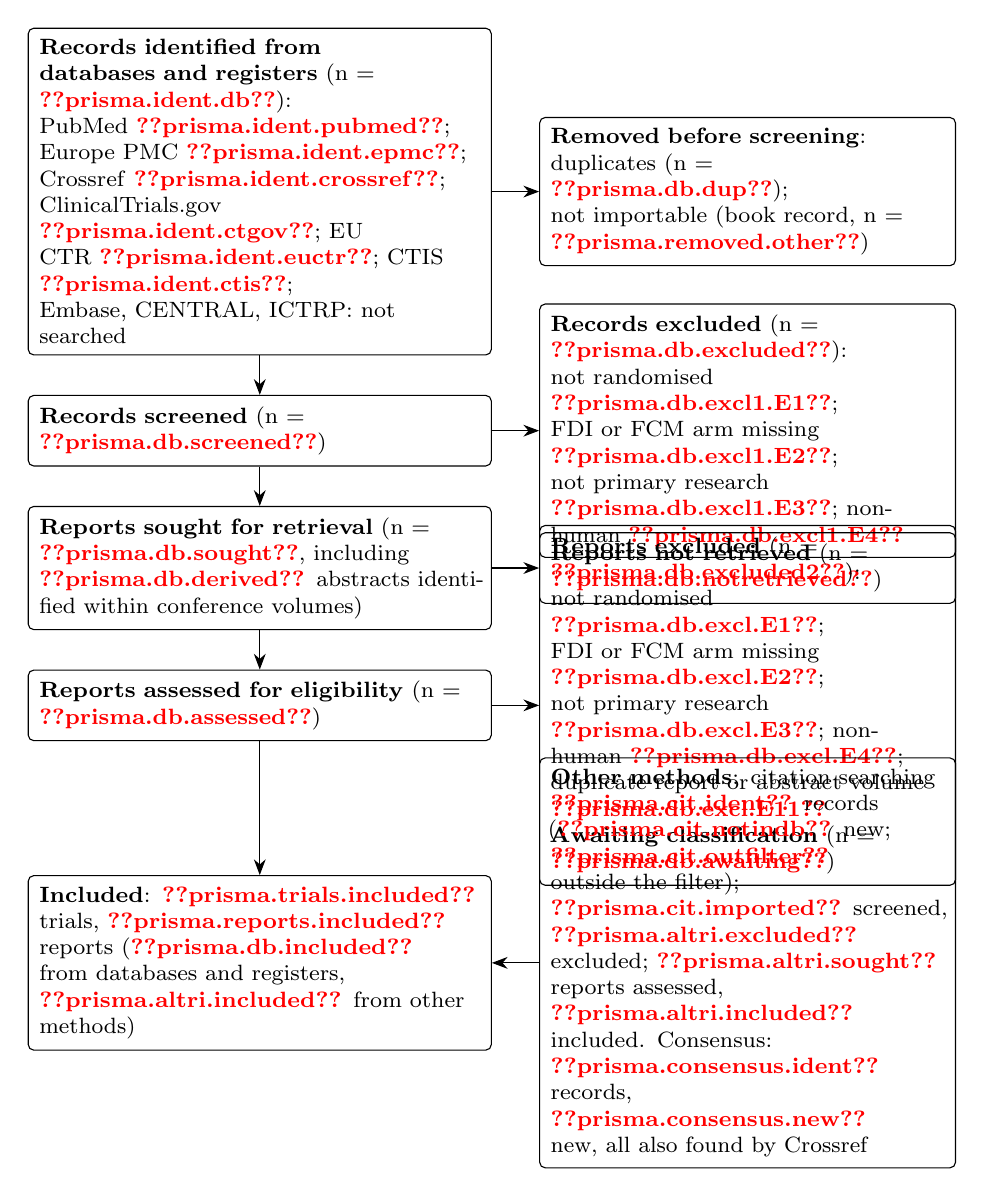
\begin{tikzpicture}[
  box/.style={draw, rounded corners=2pt, text width=5.6cm, align=left, inner sep=4pt, font=\footnotesize},
  side/.style={draw, rounded corners=2pt, text width=5.0cm, align=left, inner sep=4pt, font=\footnotesize},
  arr/.style={-{Stealth[length=2mm]}}, node distance=5mm and 6mm]
\node[box] (id) {\textbf{Records identified from databases and registers} (n = \val{prisma.ident.db}):\\
PubMed \val{prisma.ident.pubmed}; Europe PMC \val{prisma.ident.epmc}; Crossref \val{prisma.ident.crossref}; ClinicalTrials.gov \val{prisma.ident.ctgov}; EU CTR \val{prisma.ident.euctr}; CTIS \val{prisma.ident.ctis};\\ Embase, CENTRAL, ICTRP: not searched};
\node[side, right=of id] (dup) {\textbf{Removed before screening}:\\ duplicates (n = \val{prisma.db.dup});\\ not importable (book record, n = \val{prisma.removed.other})};
\node[box, below=of id] (scr) {\textbf{Records screened} (n = \val{prisma.db.screened})};
\node[side, right=of scr] (ex1) {\textbf{Records excluded} (n = \val{prisma.db.excluded}):\\ not randomised \val{prisma.db.excl1.E1}; FDI or FCM arm missing \val{prisma.db.excl1.E2}; not primary research \val{prisma.db.excl1.E3}; non-human \val{prisma.db.excl1.E4}};
\node[box, below=of scr] (sou) {\textbf{Reports sought for retrieval} (n = \val{prisma.db.sought}, including \val{prisma.db.derived} abstracts identified within conference volumes)};
\node[side, right=of sou] (nr) {\textbf{Reports not retrieved} (n = \val{prisma.db.notretrieved})};
\node[box, below=of sou] (ass) {\textbf{Reports assessed for eligibility} (n = \val{prisma.db.assessed})};
\node[side, right=of ass] (ex2) {\textbf{Reports excluded} (n = \val{prisma.db.excluded2}):\\ not randomised \val{prisma.db.excl.E1}; FDI or FCM arm missing \val{prisma.db.excl.E2}; not primary research \val{prisma.db.excl.E3}; non-human \val{prisma.db.excl.E4}; duplicate report or abstract volume \val{prisma.db.excl.E11}\\
\textbf{Awaiting classification} (n = \val{prisma.db.awaiting})};
\node[box, below=17mm of ass] (inc) {\textbf{Included}: \val{prisma.trials.included} trials, \val{prisma.reports.included} reports (\val{prisma.db.included} from databases and registers, \val{prisma.altri.included} from other methods)};
\node[side, right=of inc] (oth) {\textbf{Other methods}: citation searching \val{prisma.cit.ident} records (\val{prisma.cit.notindb} new; \val{prisma.cit.outfilter} outside the filter); \val{prisma.cit.imported} screened, \val{prisma.altri.excluded} excluded; \val{prisma.altri.sought} reports assessed, \val{prisma.altri.included} included. Consensus: \val{prisma.consensus.ident} records, \val{prisma.consensus.new} new, all also found by Crossref};
\draw[arr] (id) -- (scr); \draw[arr] (id) -- (dup);
\draw[arr] (scr) -- (sou); \draw[arr] (scr) -- (ex1);
\draw[arr] (sou) -- (ass); \draw[arr] (sou) -- (nr);
\draw[arr] (ass) -- (inc); \draw[arr] (ass) -- (ex2);
\draw[arr] (oth.west) -- (inc.east);
\end{tikzpicture}
\caption{PRISMA 2020 flow diagram. All counts are generated from the project database and search log.}\label{fig:prisma}
\end{figure}

\subsection{Characteristics of the included trials}
Table~\ref{tab:characteristics} describes the \val{trials.n} trials. Of these, \val{trials.openlabel} were open-label, \val{trials.doppio.pieno} were described as double-blind and \val{trials.parziale} as partially masked; \val{trials.pharmacosmos} were funded wholly or partly by Pharmacosmos, the manufacturer of FDI; \val{trials.vifor} involved Vifor, the manufacturer of FCM, without a funding declaration; and \val{trials.indipendenti} had no manufacturer funding (in one of these, commercially available study drugs were purchased from a distributor). A phase~I pharmacokinetic trial~\cite{R33054113} reported none of the review outcomes.

\begin{landscape}
\begin{table}[p]
\centering\scriptsize
\caption{Characteristics of the included trials (only the FDI and FCM arms are shown). $n$ = randomised. Follow-up in days; NR = not reported.}\label{tab:characteristics}
\begin{tabularx}{\linewidth}{L{2.6cm}L{2.0cm}Y L{1.9cm}L{1.3cm}L{3.1cm}L{3.1cm}L{1.0cm}L{2.1cm}}
\toprule
Trial & Country & Population & Blinding & $n$ FDI / FCM & FDI dose & FCM dose & Follow-up & Funding \\
\midrule
\tabCaratteristiche
\bottomrule
\end{tabularx}
\end{table}
\end{landscape}

\subsection{Risk of bias}
Table~\ref{tab:rob} shows the \val{rob.n} outcome-level judgements: \val{rob.low} at low risk, \val{rob.some} with some concerns and \val{rob.high} at high risk. The commonest concern in the trials contributing to the phosphate outcomes was that safety analyses followed the drug received rather than the assignment, for a few patients. Of the three judgements at high risk, two (one trial) were high because of the randomisation domain, and one was rated high because four domains had some concerns in an internally inconsistent report.

\begin{table}[htbp]
\centering\small
\caption{Risk of bias (RoB~2) by trial and outcome. D1 randomisation; D2 deviations from intended interventions; D3 missing outcome data; D4 measurement of the outcome; D5 selection of the reported result. \robL~low; \robS~some concerns; \robH~high.}\label{tab:rob}
\begin{tabular}{llcccccc}
\toprule
Trial & Outcome & D1 & D2 & D3 & D4 & D5 & Overall \\
\midrule
\tabRob
\bottomrule
\end{tabular}
\end{table}

\subsection{Hypophosphataemia}
In the primary window, FDI reduced the incidence of hypophosphataemia (\val{P1.primaria.RR.k} trials, \val{P1.primaria.RR.partecipanti} participants; risk ratio \val{P1.primaria.RR.stima}, 95\% CI \val{P1.primaria.RR.ic_inf} to \val{P1.primaria.RR.ic_sup}; $I^2$~=~\val{P1.primaria.RR.i2}\%; Figure~\ref{fig:forest}). A fifth trial had no events in either arm. The risk was \val{P1.primaria.RR.rischio_fcm_1000} per 1000 with FCM and \val{P1.primaria.RR.rischio_fdi_1000} per 1000 with FDI, a difference of \val{P1.primaria.RR.diff_1000} per 1000 (\val{P1.primaria.RR.diff_1000_inf} to \val{P1.primaria.RR.diff_1000_sup}). The estimate was unchanged by the Mantel--Haenszel model (\val{P1.primaria.affiancato-k-5.mh-effetti-fissi-senza-correzione.RR.stima}) and by the fixed-effect model. The sensitivity analyses excluding manufacturer-funded trials and restricted to low risk of bias could not be performed, because no trial qualified. In the exploratory subgroups by dose schedule, the risk ratio was \val{P1.primaria.sottogruppo-schema-dose-fdi-singola-fcm-frazionata.reml-hksj-senza-correzione.RR.stima} (\val{P1.primaria.sottogruppo-schema-dose-fdi-singola-fcm-frazionata.reml-hksj-senza-correzione.RR.ic_inf} to \val{P1.primaria.sottogruppo-schema-dose-fdi-singola-fcm-frazionata.reml-hksj-senza-correzione.RR.ic_sup}) with single-dose FDI against split-dose FCM and \val{P1.primaria.sottogruppo-schema-dose-stesso-schema.reml-hksj-senza-correzione.RR.stima} (\val{P1.primaria.sottogruppo-schema-dose-stesso-schema.reml-hksj-senza-correzione.RR.ic_inf} to \val{P1.primaria.sottogruppo-schema-dose-stesso-schema.reml-hksj-senza-correzione.RR.ic_sup}) with the same schedule in both arms (two trials each; test for difference $p$~=~\val{P1.primaria.sottogruppi-test-schema-dose.reml-hksj-senza-correzione.RR.q_p}). Subgroups by population could not be formed, because only one population had two or more trials. RAPIDIRON reported hypophosphataemia at an early visit (\val{nonusato.ctri-2020-09-027730.P1.primaria.FDI} with FDI versus \val{nonusato.ctri-2020-09-027730.P1.primaria.FCM} with FCM) and at 6~weeks after delivery (\val{nonusato.ctri-2020-09-027730.S3.estesa.FDI} versus \val{nonusato.ctri-2020-09-027730.S3.estesa.FCM}), but did not state the threshold in the article or the published protocol, so these data could not be assigned to an outcome and were not used. In the extended window two trials reported the outcome, one with events (\val{trial.P1.estesa.phosphare-ibd.fdi} versus \val{trial.P1.estesa.phosphare-ibd.fcm}) and one without (\val{trial.P1.estesa.exploriron-ckd.fdi} versus \val{trial.P1.estesa.exploriron-ckd.fcm}); the risk difference was \val{P1.estesa.RD.stima} (\val{P1.estesa.RD.ic_inf} to \val{P1.estesa.RD.ic_sup}).

No participant receiving FDI had severe hypophosphataemia (\val{S1.primaria.RD.eventi_fdi} versus \val{S1.primaria.RD.eventi_fcm}). The three trials used different thresholds: \val{soglia.S1.primaria.phosphare-ida04}~mmol/L in the two PHOSPHARE-IDA trials and \val{soglia.S1.primaria.nct03957057}~mmol/L in the post-partum trial, which measured phosphate only at 6~weeks. ExplorIRON-CKD, whose threshold was below 0.32~mmol/L and which had no events, did not enter this outcome under the threshold rule. The Peto odds ratio, from the two trials with events, was \val{S1.primaria.OR.stima} (\val{S1.primaria.OR.ic_inf} to \val{S1.primaria.OR.ic_sup}). The risk difference was \val{S1.primaria.RD.stima} (\val{S1.primaria.RD.ic_inf} to \val{S1.primaria.RD.ic_sup}; \val{S1.primaria.RD.k} trials) and \val{S1.primaria.sensibilit-3-soglia-esatta.mh-effetti-fissi-doppi-zeri-inclusi.RD.stima} (\val{S1.primaria.sensibilit-3-soglia-esatta.mh-effetti-fissi-doppi-zeri-inclusi.RD.ic_inf} to \val{S1.primaria.sensibilit-3-soglia-esatta.mh-effetti-fissi-doppi-zeri-inclusi.RD.ic_sup}) when restricted to the exact threshold. In both trials with events, this outcome was a post hoc analysis in the registry.

Hypophosphataemia persisting at the last visit of the primary window was less frequent with FDI (Mantel--Haenszel risk ratio \val{S3.primaria.RR.stima}, \val{S3.primaria.RR.ic_inf} to \val{S3.primaria.RR.ic_sup}; \val{S3.primaria.RR.k} trials; $I^2$~=~\val{S3.primaria.RR.i2}\%). The REML model alongside lost one trial to zero cells and was imprecise (\val{S3.primaria.affiancato-k-5.reml-hksj-senza-correzione.RR.stima}, \val{S3.primaria.affiancato-k-5.reml-hksj-senza-correzione.RR.ic_inf} to \val{S3.primaria.affiancato-k-5.reml-hksj-senza-correzione.RR.ic_sup}). In exploratory subgroups, the risk ratio was \val{S3.primaria.sottogruppo-schema-dose-fdi-singola-fcm-frazionata.mh-effetti-fissi-senza-correzione.RR.stima} (\val{S3.primaria.sottogruppo-schema-dose-fdi-singola-fcm-frazionata.mh-effetti-fissi-senza-correzione.RR.ic_inf} to \val{S3.primaria.sottogruppo-schema-dose-fdi-singola-fcm-frazionata.mh-effetti-fissi-senza-correzione.RR.ic_sup}) with single-dose FDI against split-dose FCM and \val{S3.primaria.sottogruppo-schema-dose-stesso-schema.mh-effetti-fissi-senza-correzione.RR.stima} (\val{S3.primaria.sottogruppo-schema-dose-stesso-schema.mh-effetti-fissi-senza-correzione.RR.ic_inf} to \val{S3.primaria.sottogruppo-schema-dose-stesso-schema.mh-effetti-fissi-senza-correzione.RR.ic_sup}) with the same schedule (test for difference $p$~=~\val{S3.primaria.sottogruppi-test-schema-dose.mh-effetti-fissi-senza-correzione.RR.q_p}); with two trials per subgroup and a classification written after the data were known, this is hypothesis-generating only.

At day~35, serum phosphate changed little from baseline with FDI and fell with FCM (mean difference \val{S4.primaria.MD.stima}~mmol/L, \val{S4.primaria.MD.ic_inf} to \val{S4.primaria.MD.ic_sup}; \val{S4.primaria.MD.k} trials, both funded by the manufacturer of FDI). Four further trials reported phosphate in forms that could not be pooled: values at day~35 without the number of participants per visit, medians, and a least-squares mean change without dispersion in an abstract. In the trial without manufacturer funding, which measured phosphate only at 6~weeks, median values were almost identical in the two arms.

Hypophosphataemia at the wide threshold was reported by single trials only: \val{trial.S2.primaria.nct03957057.fdi} versus \val{trial.S2.primaria.nct03957057.fcm} in the post-partum trial (threshold \val{soglia.S2.primaria.nct03957057}~mmol/L, at 6~weeks) and, in the extended window, \val{trial.S2.estesa.exploriron-ckd.fdi} versus \val{trial.S2.estesa.exploriron-ckd.fcm} in ExplorIRON-CKD (threshold \val{soglia.S2.estesa.exploriron-ckd}~mmol/L, episodes reported as adverse events).

\begin{figure}[htbp]
\centering
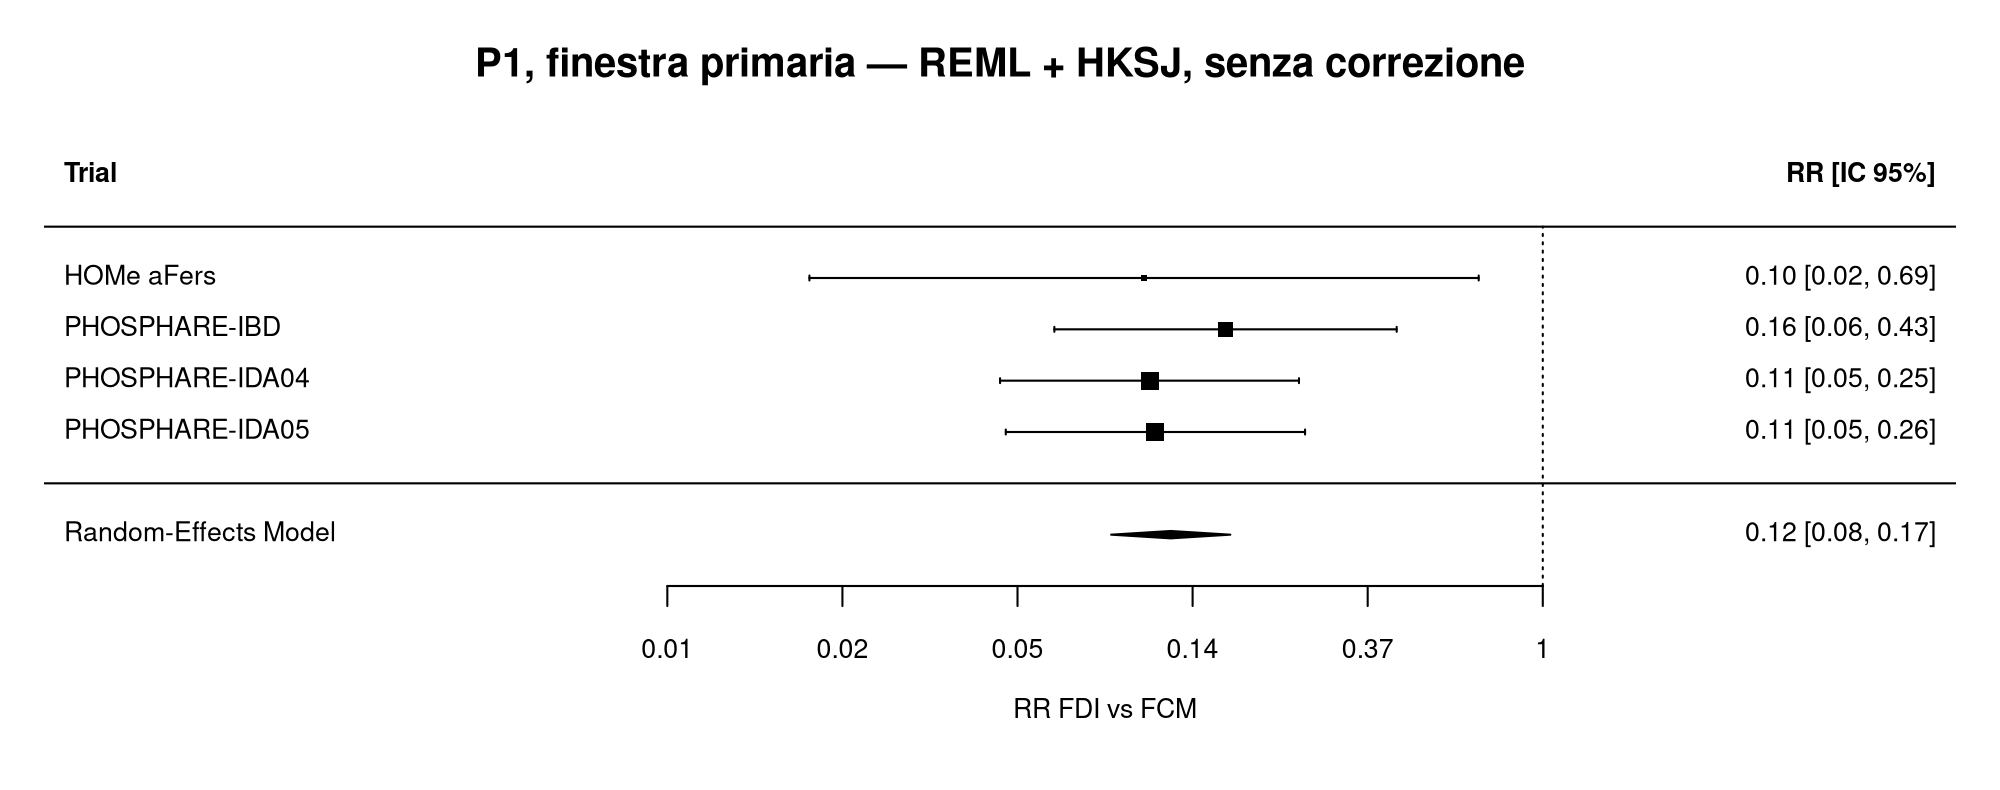
\includegraphics[width=0.9\textwidth]{P1-primaria-reml.png}\\[2pt]
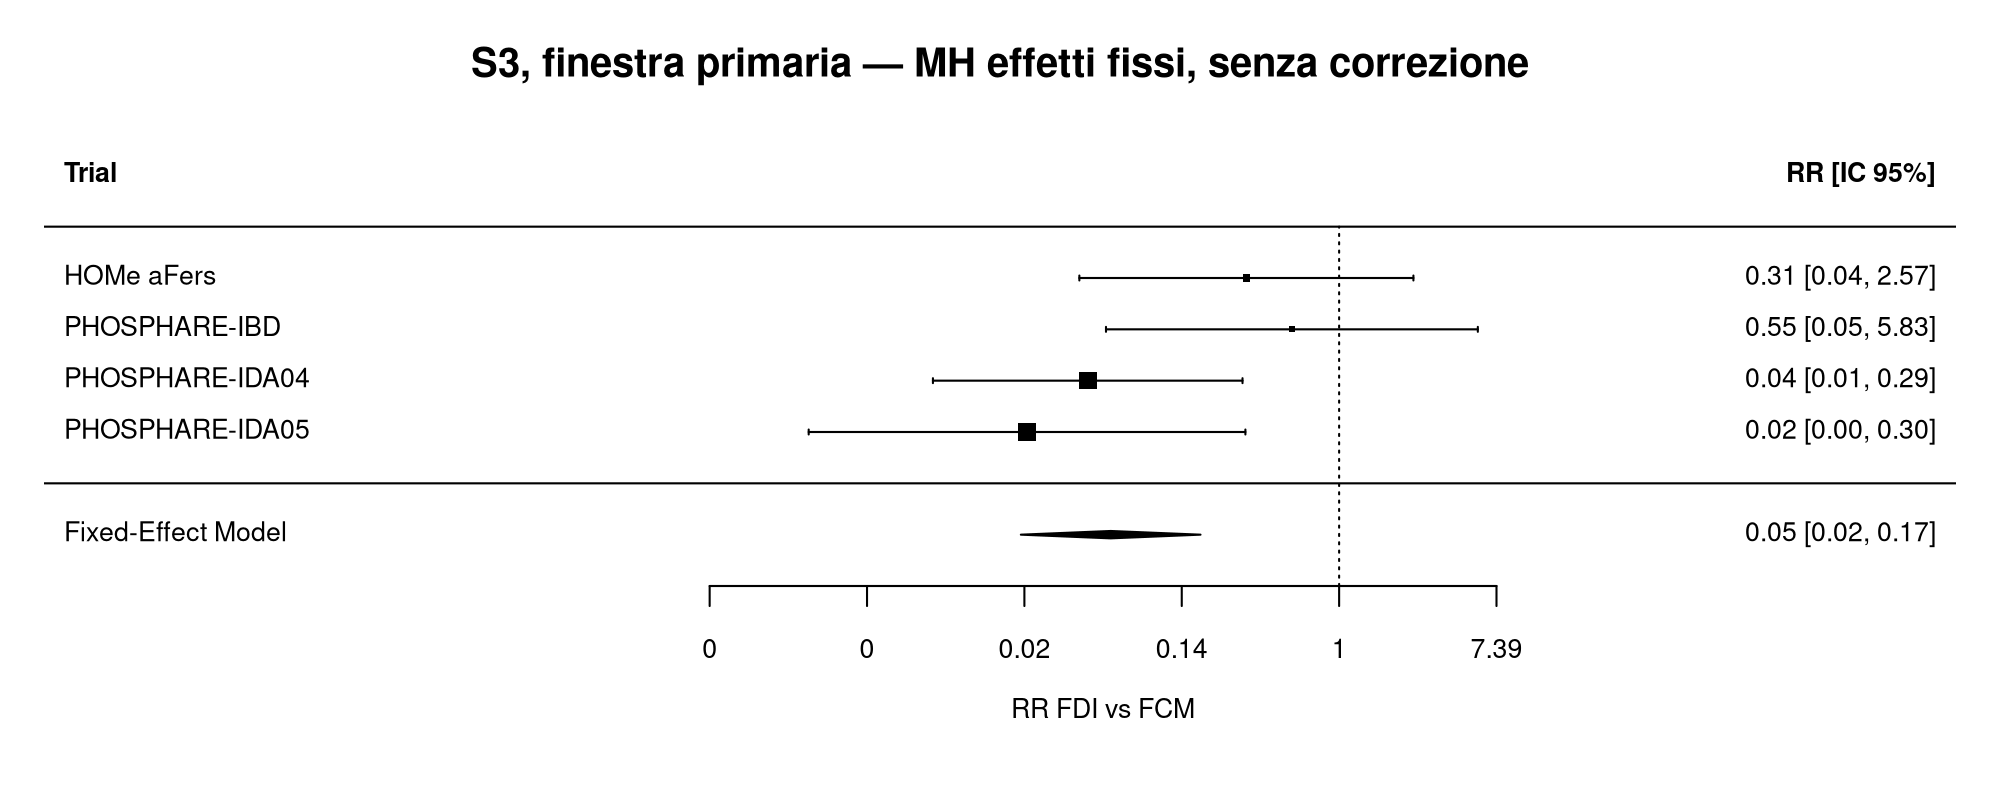
\includegraphics[width=0.9\textwidth]{S3-primaria-mh.png}\\[2pt]
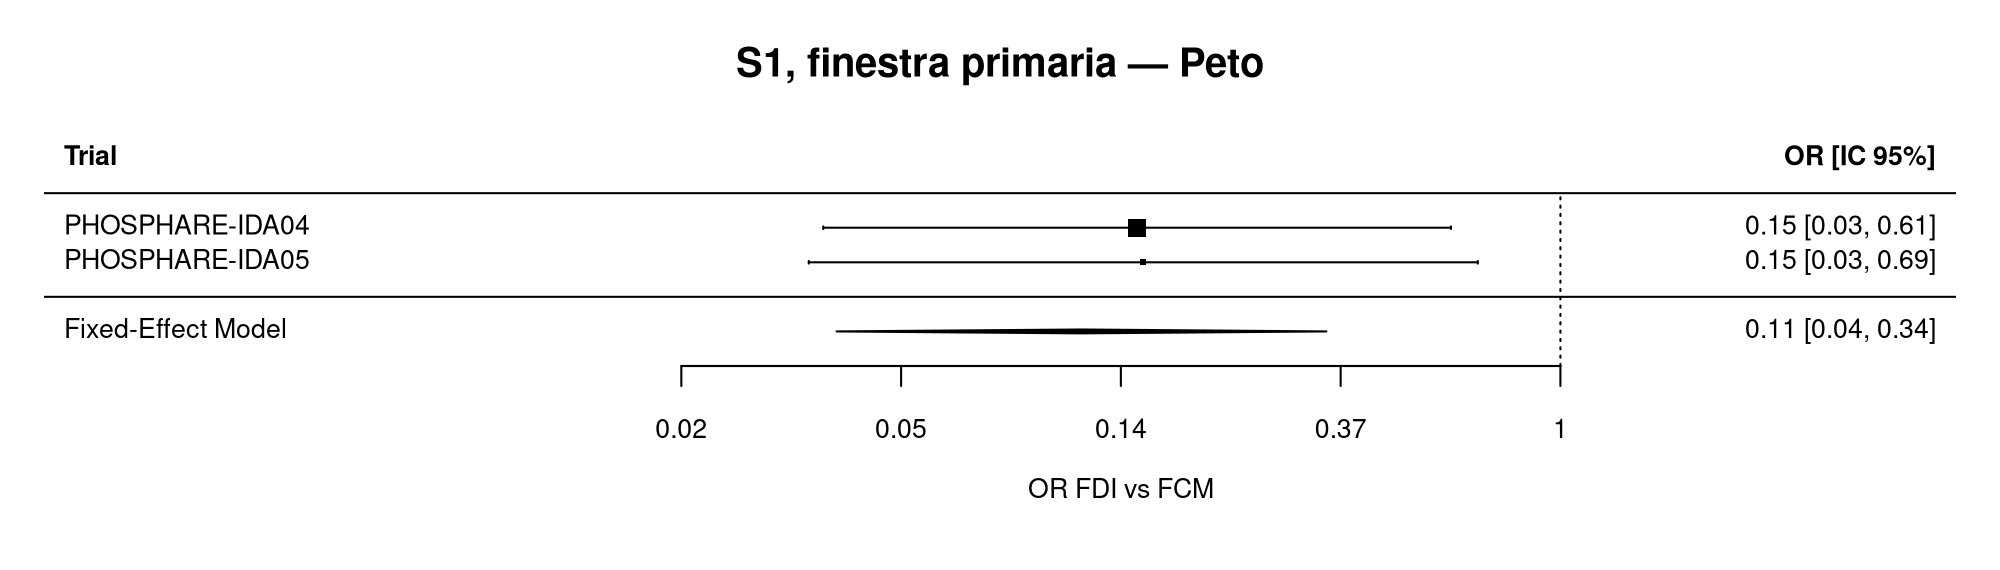
\includegraphics[width=0.9\textwidth]{S1-primaria-peto.png}\\[2pt]
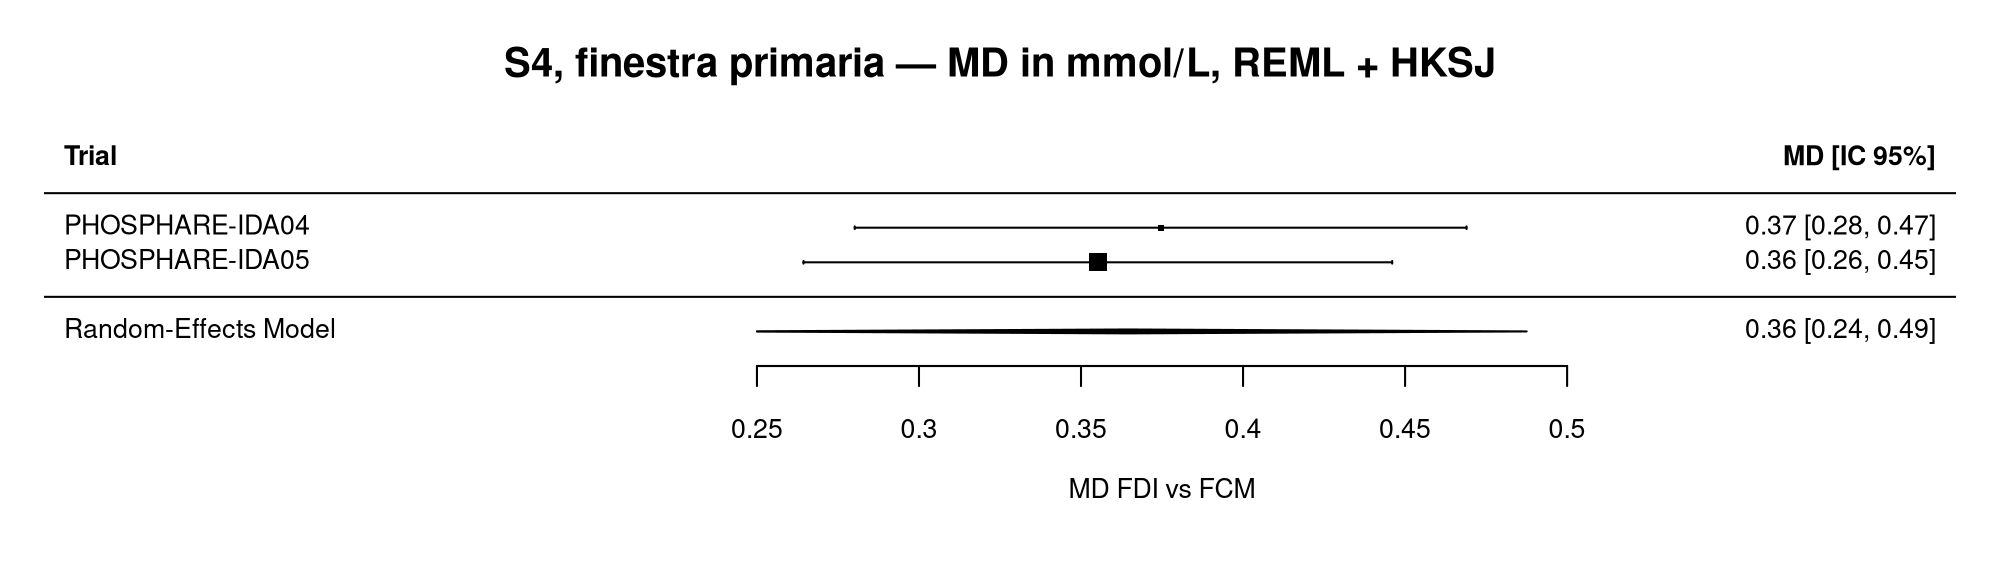
\includegraphics[width=0.9\textwidth]{S4-primaria-reml.png}
\caption{Forest plots of the main analyses: hypophosphataemia (REML--HKSJ, risk ratio), persistent hypophosphataemia (Mantel--Haenszel, risk ratio), severe hypophosphataemia (Peto odds ratio) and change in serum phosphate at day~35 (mean difference, mmol/L). Effects are FDI relative to FCM.}\label{fig:forest}
\end{figure}

\subsection{Hypersensitivity}
Serious or severe hypersensitivity reactions were rare in the primary window (\val{S6.primaria.RR.eventi_fdi} with FDI versus \val{S6.primaria.RR.eventi_fcm} with FCM). The Mantel--Haenszel risk ratio was \val{S6.primaria.RR.stima} (\val{S6.primaria.RR.ic_inf} to \val{S6.primaria.RR.ic_sup}; \val{S6.primaria.RR.k} trials with events), and the Mantel--Haenszel risk difference, including double-zero trials, was \val{S6.primaria.sensibilit-mh-effetti-fissi-doppi-zeri-inclusi.mh-effetti-fissi-doppi-zeri-inclusi.RD.stima} (\val{S6.primaria.sensibilit-mh-effetti-fissi-doppi-zeri-inclusi.mh-effetti-fissi-doppi-zeri-inclusi.RD.ic_inf} to \val{S6.primaria.sensibilit-mh-effetti-fissi-doppi-zeri-inclusi.mh-effetti-fissi-doppi-zeri-inclusi.RD.ic_sup}; \val{S6.primaria.sensibilit-mh-effetti-fissi-doppi-zeri-inclusi.mh-effetti-fissi-doppi-zeri-inclusi.RD.k} trials). Definitions ranged from protocol-defined serious or severe reactions, whose criteria were not available to us, to externally adjudicated infusion-related serious adverse events without severity criteria.

Any hypersensitivity or infusion reaction was not pooled. The two trials used different definitions and pointed in opposite directions:
\begin{itemize}
\item \val{trial.S7.primaria.nct03957057.fdi} versus \val{trial.S7.primaria.nct03957057.fcm} in the post-partum trial;
\item \val{trial.S7.primaria.rapidiron.fdi} versus \val{trial.S7.primaria.rapidiron.fcm} in RAPIDIRON (risk ratio \val{trial.S7.primaria.rapidiron.rr}, \val{trial.S7.primaria.rapidiron.rr_inf} to \val{trial.S7.primaria.rapidiron.rr_sup}).
\end{itemize}

\subsection{Cardiovascular events, osteomalacia and fractures}
No trial reported adjudicated cardiovascular events. Serious cardiac or vascular adverse events were zero in both arms of the two trials reporting them in the primary window (\val{S8b.primaria.RD.eventi_fdi} versus \val{S8b.primaria.RD.eventi_fcm}), so no effect could be estimated. In the extended window the risk difference was \val{S8b.estesa.RD.stima} (\val{S8b.estesa.RD.ic_inf} to \val{S8b.estesa.RD.ic_sup}; \val{S8b.estesa.RD.k} trials, \val{S8b.estesa.RD.eventi_fdi} versus \val{S8b.estesa.RD.eventi_fcm}). ExplorIRON-CKD listed one serious atrial fibrillation event in the FDI arm by event rather than by patient, which was not extracted, and one trial prespecified an adjudicated cardiovascular composite that it did not report. No trial reported osteomalacia or fractures.

\subsection{Registered and published trials}
Of the \val{reg.trials.withregistry} included trials whose registry records we retrieved, all \val{reg.trials.withregistry.published} had been published. One registered head-to-head trial (\val{reg.awaiting.ids}) had no results; its registry status was unknown, last reported as recruiting, and its estimated completion date had passed only recently. It is listed as awaiting classification. The registry of one further included trial (CTRI) was not searched, and ICTRP was not searched.

\subsection{Certainty of the evidence}
Table~\ref{tab:sof} summarises the findings. Hypophosphataemia (in both windows), severe and persistent hypophosphataemia and the change in phosphate were of low certainty, downgraded for risk of bias and imprecision. For the primary outcome, imprecision was downgraded only because the number of events was below the optimal information size, while the confidence interval was far from the null. All other outcomes, including hypophosphataemia at the wide threshold, were of very low certainty.

\begin{landscape}
\begin{table}[p]
\centering\scriptsize
\caption{Summary of findings: FDI compared with FCM in adults with iron deficiency. Risks per 1000 participants. The FCM risk is the crude pooled risk in the FCM arms of the trials in each model; the FDI risk is model-derived from it and from the relative effect (for severe hypophosphataemia no event was observed with FDI).}\label{tab:sof}
\begin{tabularx}{\linewidth}{L{4.4cm}L{1.9cm}L{1.6cm}L{1.3cm}L{3.2cm}Y L{1.3cm}}
\toprule
Outcome & Trials (participants) & Risk with FCM & Risk with FDI & Difference per 1000 (95\% CI) & Relative effect (95\% CI) & Certainty \\
\midrule
\tabSof
\bottomrule
\end{tabularx}
\end{table}
\end{landscape}

% ======================================================================= DISCUSSION
\section{Discussion}

\subsection{Main findings}
In head-to-head randomised trials, FDI may reduce the incidence of hypophosphataemia, of severe hypophosphataemia and of hypophosphataemia persisting at the end of the primary window compared with FCM. The effect on the primary outcome was large and consistent across individual trials that used identical doses of the two drugs and trials that used different regimens, although the pooled same-schedule subgroup was imprecise. Its certainty is low because of risk-of-bias concerns in all contributing trials and because the number of events was below the optimal information size, which we applied strictly; the confidence interval excludes the null by a wide margin. All trials contributing to the pooled estimates for hypophosphataemia, persistent hypophosphataemia and change in phosphate were funded by the manufacturer of FDI; we did not downgrade for this, but no independent trial reported the outcome as defined: the two independent trials that measured phosphate used a single late measurement or did not state the threshold. Evidence on hypersensitivity and cardiovascular safety is very uncertain. No head-to-head trial has reported osteomalacia or fractures, the clinical consequences that motivate concern about hypophosphataemia.

\subsection{Comparison with previous syntheses}
Previous syntheses reached their estimates mainly through network, indirect or study-level comparisons~\cite{Bellos2020,Schaefer2021,Kennedy2023,Pollock2022,Divers2026,Azevedo2026}. Our review restricts the evidence to direct randomisation. This reduces the number of trials, but it removes the exchangeability assumption between trials against different comparators. The direction of our findings on hypophosphataemia is consistent with the syntheses that addressed it~\cite{Bellos2020,Schaefer2021,Azevedo2026}. We do not compare magnitudes, because the populations, thresholds and methods differ.

\subsection{Strengths and limitations}
\textbf{Strengths.}
\begin{itemize}
\item Independent duplicate screening, extraction, risk-of-bias assessment and GRADE rating, with author adjudication of discordances.
\item Author verification against the source of every analysed data row.
\item Arm-level data taken from registries as well as articles.
\item Aggregate numbers produced only by versioned scripts, so every estimate can be traced to a data row and page.
\end{itemize}

\textbf{Limitations.}
\begin{itemize}
\item The protocol was frozen after the repository already held unstructured notes and extractions on some trials, and it was not registered prospectively.
\item Several deviations were decided after seeing the results: the main model with zero cells, the correction of the pooling rule and the new risk-difference rule, the application of the threshold rule to severe hypophosphataemia, the inclusion of a double-zero trial in the extended window of the primary outcome, not pooling any hypersensitivity, the descriptive registered-versus-published comparison, and the subgroup classification. All are declared; for zero cells the alternative models are reported, and any hypersensitivity is reported trial by trial.
\item Embase, Cochrane CENTRAL and WHO ICTRP were not searched, so trials indexed only there, and registered trials outside ClinicalTrials.gov and the EU registers, may have been missed; the publication-bias rating is provisional for this reason.
\item Few trials contributed to each outcome, and the trials informing the pooled estimates for hypophosphataemia, persistent hypophosphataemia and change in phosphate were all funded by one manufacturer.
\item Thresholds for severe and wide-threshold hypophosphataemia differed between trials, and the risk difference for severe hypophosphataemia includes a trial that measured phosphate only at 6~weeks.
\item Eligibility evidence sheets were prepared by a single agent run, and the eligibility proposals were approved in blocks.
\item The hypersensitivity outcomes rest on heterogeneous definitions.
\item Automated agents performed the first pass of every step, and concordant exclusions at title and abstract, as well as concordant risk-of-bias and GRADE judgements, were not reviewed by an author. We mitigated this with duplicate independent runs, algorithmic checks and author adjudication of discordances, but it remains a methodological novelty.
\end{itemize}

\subsection{Implications for research}
Future head-to-head trials should:
\begin{itemize}
\item be independent of manufacturers;
\item define hypophosphataemia at prespecified thresholds and time points;
\item follow participants long enough to capture musculoskeletal consequences;
\item use standard criteria for serious hypersensitivity.
\end{itemize}

\section{Conclusions}
In head-to-head randomised trials in adults with iron deficiency, FDI may reduce the incidence of hypophosphataemia compared with FCM (low-certainty evidence). The comparative effects on hypersensitivity and cardiovascular events are very uncertain, and no head-to-head trial has reported osteomalacia or fractures.

\section*{Declarations}
\noindent\textbf{Funding.} This work received no specific funding.\\
\textbf{Competing interests.} The authors declare no competing interests.\\
\textbf{Ethics.} This review used only published or registry-posted aggregate data; ethical approval and consent were not required.\\
\textbf{Data and code availability.} The frozen protocol, search logs, screening decisions, arm-level extraction files, risk-of-bias and GRADE files, the analysis script (\texttt{50-Metanalisi/analisi.R}) and all its outputs, the agent instructions and an export of the selection database are openly available at \url{https://github.com/filippobuscemi11463-sketch/FDI-FCM-metaanalysis}. Full texts and abstracts of the included reports are not redistributed.\\
\textbf{Use of AI tools.} Large-language-model agents (Claude, Anthropic, via Claude Code) were used for duplicate screening, extraction, risk-of-bias and GRADE assessments, and for drafting code and text, under the procedures described in Methods. Concordant exclusions at title and abstract screening and concordant risk-of-bias and GRADE judgements were accepted without author review; eligibility proposals prepared by a single agent run were approved by an author; discordant and uncertain records, extracted values and judgements were decided by an author, who also verified every data row selected for analysis. The authors take full responsibility for the content.\\
\textbf{Author contributions.} F.B. and P.B. contributed equally to this work. Both authors approved the final manuscript.

\bibliographystyle{unsrtnat}
\bibliography{generati/refs-trial,generati/refs-altri}

\end{document}
